
%% bare_conf.tex
%% V1.3
%% 2007/01/11
%% by Michael Shell
%% See:
%% http://www.michaelshell.org/
%% for current contact information.
%%
%% This is a skeleton file demonstrating the use of IEEEtran.cls
%% (requires IEEEtran.cls version 1.7 or later) with an IEEE conference paper.
%%
%% Support sites:
%% http://www.michaelshell.org/tex/ieeetran/
%% http://www.ctan.org/tex-archive/macros/latex/contrib/IEEEtran/
%% and
%% http://www.ieee.org/

%%*************************************************************************
%% Legal Notice:
%% This code is offered as-is without any warranty either expressed or
%% implied; without even the implied warranty of MERCHANTABILITY or
%% FITNESS FOR A PARTICULAR PURPOSE!
%% User assumes all risk.
%% In no event shall IEEE or any contributor to this code be liable for
%% any damages or losses, including, but not limited to, incidental,
%% consequential, or any other damages, resulting from the use or misuse
%% of any information contained here.
%%
%% All comments are the opinions of their respective authors and are not
%% necessarily endorsed by the IEEE.
%%
%% This work is distributed under the LaTeX Project Public License (LPPL)
%% ( http://www.latex-project.org/ ) version 1.3, and may be freely used,
%% distributed and modified. A copy of the LPPL, version 1.3, is included
%% in the base LaTeX documentation of all distributions of LaTeX released
%% 2003/12/01 or later.
%% Retain all contribution notices and credits.
%% ** Modified files should be clearly indicated as such, including  **
%% ** renaming them and changing author support contact information. **
%%
%% File list of work: IEEEtran.cls, IEEEtran_HOWTO.pdf, bare_adv.tex,
%%                    bare_conf.tex, bare_jrnl.tex, bare_jrnl_compsoc.tex
%%*************************************************************************

% *** Authors should verify (and, if needed, correct) their LaTeX system  ***
% *** with the testflow diagnostic prior to trusting their LaTeX platform ***
% *** with production work. IEEE's font choices can trigger bugs that do  ***
% *** not appear when using other class files.                            ***
% The testflow support page is at:
% http://www.michaelshell.org/tex/testflow/



% Note that the a4paper option is mainly intended so that authors in
% countries using A4 can easily print to A4 and see how their papers will
% look in print - the typesetting of the document will not typically be
% affected with changes in paper size (but the bottom and side margins will).
% Use the testflow package mentioned above to verify correct handling of
% both paper sizes by the user's LaTeX system.
%
% Also note that the "draftcls" or "draftclsnofoot", not "draft", option
% should be used if it is desired that the figures are to be displayed in
% draft mode.
%
%\documentclass[10pt, conference]{IEEEtran}

\documentclass[conference]{IEEEtran}

%compsocconf
% Add the compsocconf option for Computer Society conferences.
%
% If IEEEtran.cls has not been installed into the LaTeX system files,
% manually specify the path to it like:
% \documentclass[conference]{../sty/IEEEtran}





% Some very useful LaTeX packages include:
% (uncomment the ones you want to load)


% *** MISC UTILITY PACKAGES ***
%
%\usepackage{ifpdf}
% Heiko Oberdiek's ifpdf.sty is very useful if you need conditional
% compilation based on whether the output is pdf or dvi.
% usage:
% \ifpdf
%   % pdf code
% \else
%   % dvi code
% \fi
% The latest version of ifpdf.sty can be obtained from:
% http://www.ctan.org/tex-archive/macros/latex/contrib/oberdiek/
% Also, note that IEEEtran.cls V1.7 and later provides a builtin
% \ifCLASSINFOpdf conditional that works the same way.
% When switching from latex to pdflatex and vice-versa, the compiler may
% have to be run twice to clear warning/error messages.






% *** CITATION PACKAGES ***
%
%\usepackage{cite}
% cite.sty was written by Donald Arseneau
% V1.6 and later of IEEEtran pre-defines the format of the cite.sty package
% \cite{} output to follow that of IEEE. Loading the cite package will
% result in citation numbers being automatically sorted and properly
% "compressed/ranged". e.g., [1], [9], [2], [7], [5], [6] without using
% cite.sty will become [1], [2], [5]--[7], [9] using cite.sty. cite.sty's
% \cite will automatically add leading space, if needed. Use cite.sty's
% noadjust option (cite.sty V3.8 and later) if you want to turn this off.
% cite.sty is already installed on most LaTeX systems. Be sure and use
% version 4.0 (2003-05-27) and later if using hyperref.sty. cite.sty does
% not currently provide for hyperlinked citations.
% The latest version can be obtained at:
% http://www.ctan.org/tex-archive/macros/latex/contrib/cite/
% The documentation is contained in the cite.sty file itself.






% *** GRAPHICS RELATED PACKAGES ***
%
\ifCLASSINFOpdf
  % \usepackage[pdftex]{graphicx}
  % declare the path(s) where your graphic files are
  % \graphicspath{{../pdf/}{../jpeg/}}
  % and their extensions so you won't have to specify these with
  % every instance of \includegraphics
  % \DeclareGraphicsExtensions{.pdf,.jpeg,.png}
\else
  % or other class option (dvipsone, dvipdf, if not using dvips). graphicx
  % will default to the driver specified in the system graphics.cfg if no
  % driver is specified.
  % \usepackage[dvips]{graphicx}
  % declare the path(s) where your graphic files are
  % \graphicspath{{../eps/}}
  % and their extensions so you won't have to specify these with
  % every instance of \includegraphics
  % \DeclareGraphicsExtensions{.eps}
\fi
% graphicx was written by David Carlisle and Sebastian Rahtz. It is
% required if you want graphics, photos, etc. graphicx.sty is already
% installed on most LaTeX systems. The latest version and documentation can
% be obtained at:
% http://www.ctan.org/tex-archive/macros/latex/required/graphics/
% Another good source of documentation is "Using Imported Graphics in
% LaTeX2e" by Keith Reckdahl which can be found as epslatex.ps or
% epslatex.pdf at: http://www.ctan.org/tex-archive/info/
%
% latex, and pdflatex in dvi mode, support graphics in encapsulated
% postscript (.eps) format. pdflatex in pdf mode supports graphics
% in .pdf, .jpeg, .png and .mps (metapost) formats. Users should ensure
% that all non-photo figures use a vector format (.eps, .pdf, .mps) and
% not a bitmapped formats (.jpeg, .png). IEEE frowns on bitmapped formats
% which can result in "jaggedy"/blurry rendering of lines and letters as
% well as large increases in file sizes.
%
% You can find documentation about the pdfTeX application at:
% http://www.tug.org/applications/pdftex





% *** MATH PACKAGES ***
%
%\usepackage[cmex10]{amsmath}
% A popular package from the American Mathematical Society that provides
% many useful and powerful commands for dealing with mathematics. If using
% it, be sure to load this package with the cmex10 option to ensure that
% only type 1 fonts will utilized at all point sizes. Without this option,
% it is possible that some math symbols, particularly those within
% footnotes, will be rendered in bitmap form which will result in a
% document that can not be IEEE Xplore compliant!
%
% Also, note that the amsmath package sets \interdisplaylinepenalty to 10000
% thus preventing page breaks from occurring within multiline equations. Use:
%\interdisplaylinepenalty=2500
% after loading amsmath to restore such page breaks as IEEEtran.cls normally
% does. amsmath.sty is already installed on most LaTeX systems. The latest
% version and documentation can be obtained at:
% http://www.ctan.org/tex-archive/macros/latex/required/amslatex/math/





% *** SPECIALIZED LIST PACKAGES ***
%
%\usepackage{algorithmic}
% algorithmic.sty was written by Peter Williams and Rogerio Brito.
% This package provides an algorithmic environment fo describing algorithms.
% You can use the algorithmic environment in-text or within a figure
% environment to provide for a floating algorithm. Do NOT use the algorithm
% floating environment provided by algorithm.sty (by the same authors) or
% algorithm2e.sty (by Christophe Fiorio) as IEEE does not use dedicated
% algorithm float types and packages that provide these will not provide
% correct IEEE style captions. The latest version and documentation of
% algorithmic.sty can be obtained at:
% http://www.ctan.org/tex-archive/macros/latex/contrib/algorithms/
% There is also a support site at:
% http://algorithms.berlios.de/index.html
% Also of interest may be the (relatively newer and more customizable)
% algorithmicx.sty package by Szasz Janos:
% http://www.ctan.org/tex-archive/macros/latex/contrib/algorithmicx/




% *** ALIGNMENT PACKAGES ***
%
%\usepackage{array}
% Frank Mittelbach's and David Carlisle's array.sty patches and improves
% the standard LaTeX2e array and tabular environments to provide better
% appearance and additional user controls. As the default LaTeX2e table
% generation code is lacking to the point of almost being broken with
% respect to the quality of the end results, all users are strongly
% advised to use an enhanced (at the very least that provided by array.sty)
% set of table tools. array.sty is already installed on most systems. The
% latest version and documentation can be obtained at:
% http://www.ctan.org/tex-archive/macros/latex/required/tools/


%\usepackage{mdwmath}
%\usepackage{mdwtab}
% Also highly recommended is Mark Wooding's extremely powerful MDW tools,
% especially mdwmath.sty and mdwtab.sty which are used to format equations
% and tables, respectively. The MDWtools set is already installed on most
% LaTeX systems. The lastest version and documentation is available at:
% http://www.ctan.org/tex-archive/macros/latex/contrib/mdwtools/


% IEEEtran contains the IEEEeqnarray family of commands that can be used to
% generate multiline equations as well as matrices, tables, etc., of high
% quality.


%\usepackage{eqparbox}
% Also of notable interest is Scott Pakin's eqparbox package for creating
% (automatically sized) equal width boxes - aka "natural width parboxes".
% Available at:
% http://www.ctan.org/tex-archive/macros/latex/contrib/eqparbox/





% *** SUBFIGURE PACKAGES ***
%\usepackage[tight,footnotesize]{subfigure}
% subfigure.sty was written by Steven Douglas Cochran. This package makes it
% easy to put subfigures in your figures. e.g., "Figure 1a and 1b". For IEEE
% work, it is a good idea to load it with the tight package option to reduce
% the amount of white space around the subfigures. subfigure.sty is already
% installed on most LaTeX systems. The latest version and documentation can
% be obtained at:
% http://www.ctan.org/tex-archive/obsolete/macros/latex/contrib/subfigure/
% subfigure.sty has been superceeded by subfig.sty.



%\usepackage[caption=false]{caption}
%\usepackage[font=footnotesize]{subfig}
% subfig.sty, also written by Steven Douglas Cochran, is the modern
% replacement for subfigure.sty. However, subfig.sty requires and
% automatically loads Axel Sommerfeldt's caption.sty which will override
% IEEEtran.cls handling of captions and this will result in nonIEEE style
% figure/table captions. To prevent this problem, be sure and preload
% caption.sty with its "caption=false" package option. This is will preserve
% IEEEtran.cls handing of captions. Version 1.3 (2005/06/28) and later
% (recommended due to many improvements over 1.2) of subfig.sty supports
% the caption=false option directly:
%\usepackage[caption=false,font=footnotesize]{subfig}
%
% The latest version and documentation can be obtained at:
% http://www.ctan.org/tex-archive/macros/latex/contrib/subfig/
% The latest version and documentation of caption.sty can be obtained at:
% http://www.ctan.org/tex-archive/macros/latex/contrib/caption/




% *** FLOAT PACKAGES ***
%
%\usepackage{fixltx2e}
% fixltx2e, the successor to the earlier fix2col.sty, was written by
% Frank Mittelbach and David Carlisle. This package corrects a few problems
% in the LaTeX2e kernel, the most notable of which is that in current
% LaTeX2e releases, the ordering of single and double column floats is not
% guaranteed to be preserved. Thus, an unpatched LaTeX2e can allow a
% single column figure to be placed prior to an earlier double column
% figure. The latest version and documentation can be found at:
% http://www.ctan.org/tex-archive/macros/latex/base/



%\usepackage{stfloats}
% stfloats.sty was written by Sigitas Tolusis. This package gives LaTeX2e
% the ability to do double column floats at the bottom of the page as well
% as the top. (e.g., "\begin{figure*}[!b]" is not normally possible in
% LaTeX2e). It also provides a command:
%\fnbelowfloat
% to enable the placement of footnotes below bottom floats (the standard
% LaTeX2e kernel puts them above bottom floats). This is an invasive package
% which rewrites many portions of the LaTeX2e float routines. It may not work
% with other packages that modify the LaTeX2e float routines. The latest
% version and documentation can be obtained at:
% http://www.ctan.org/tex-archive/macros/latex/contrib/sttools/
% Documentation is contained in the stfloats.sty comments as well as in the
% presfull.pdf file. Do not use the stfloats baselinefloat ability as IEEE
% does not allow \baselineskip to stretch. Authors submitting work to the
% IEEE should note that IEEE rarely uses double column equations and
% that authors should try to avoid such use. Do not be tempted to use the
% cuted.sty or midfloat.sty packages (also by Sigitas Tolusis) as IEEE does
% not format its papers in such ways.





% *** PDF, URL AND HYPERLINK PACKAGES ***
%
%\usepackage{url}
% url.sty was written by Donald Arseneau. It provides better support for
% handling and breaking URLs. url.sty is already installed on most LaTeX
% systems. The latest version can be obtained at:
% http://www.ctan.org/tex-archive/macros/latex/contrib/misc/
% Read the url.sty source comments for usage information. Basically,
% \url{my_url_here}.


\usepackage{mathptmx}
\usepackage{microtype}

\usepackage{balance}

\usepackage{ulem}

\usepackage{listings}
\normalem
%\usepackage{latex8}
%\usepackage{times}
\usepackage{epsf}
\usepackage{ctable}
%\usepackage{latexsym}
%\usepackage{tweaklist}
%\usepackage{rotating}
\usepackage{listings}
%\usepackage{alltt}
%\usepackage{fvrb-ex}
\usepackage{graphicx}
\usepackage{url}
\usepackage{float}
%\floatstyle{boxed}
\restylefloat{figure}


% *** Do not adjust lengths that control margins, column widths, etc. ***
% *** Do not use packages that alter fonts (such as pslatex).         ***
% There should be no need to do such things with IEEEtran.cls V1.6 and later.
% (Unless specifically asked to do so by the journal or conference you plan
% to submit to, of course. )



\usepackage{xspace}
\newcommand{\cf}{\hbox{\emph{cf.}}\xspace}
\newcommand{\deletia}{\ldots [deletia] \ldots}
\newcommand{\etal}{\hbox{\emph{et al.}}\xspace}
\newcommand{\eg}{\hbox{\emph{e.g.,}}\xspace}
\newcommand{\ie}{\hbox{\emph{i.e.,}}\xspace}
\newcommand{\st}{\hbox{\emph{s.t.}}\xspace}
\newcommand{\wrt}{\hbox{\emph{w.r.t.}}\xspace}
\newcommand{\viz}{\hbox{\emph{viz.}}\xspace}

\newcommand{\todo}[1]{\textcolor{red}{TODO: #1}\PackageWarning{TODO:}{#1!}}

\usepackage{amsmath}
\usepackage{booktabs}
\usepackage{multirow}
\usepackage{textcomp}

\usepackage[T1]{fontenc}
\usepackage{array}

\newtheorem{Definition}{Definition}
\newtheorem{Claim}{Claim}
\newtheorem{Lemma}{Lemma}
\newtheorem{Theorem}{Theorem}
\newtheorem{Property}{Property}
\newcommand{\code}[1]{{\scriptsize\textsf{#1}}}
\newcommand{\tool}{Dnn4C}

%\newcommand{\todo}[1]{\textcolor{red}{TODO: #1}\PackageWarning{TODO:}{#1!}}

\lstset{
    language={}, emph={},
    mathescape=false, escapechar=@,
    basicstyle=\scriptsize\sffamily,
    numberstyle=\scriptsize\sffamily,
    emphstyle=\bfseries,
    numbers=left, stepnumber=1, %numbersep=7pt,
    frame=single, xleftmargin=4pt, xrightmargin=4pt, framexleftmargin=0pt, framexrightmargin=0pt,  %xleftmargin=11pt
    columns=flexible, breaklines=true, showspaces=false, showstringspaces=true, showtabs=false, tabsize=4
}

\hyphenation{op-tical net-works semi-conduc-tor}

\pagenumbering{arabic}

\IEEEoverridecommandlockouts

\begin{document}

\setlength{\pdfpagewidth}{8.5in}
\setlength{\pdfpageheight}{11in}

% paper title
% can use linebreaks \\ within to get better formatting as desired
%\title{Bare Demo of IEEEtran.cls for IEEECS Conferences}

%\title{Statistical Learning of API Mappings for Code Migration\\ with Vector Transformations}

%\title{Exploring API Embedding in Source Code\\ and Its Applications}
%\title{Exploring API Embedding for API Usages\\ and Applications}

\title{A Deep Neural Network Language Model with Contexts for Source Code}
%with\\ Syntactic and Semantic Contexts for Java Source Code}


% author names and affiliations
% use a multiple column layout for up to two different
% affiliations

\author{\IEEEauthorblockN{Anh Tuan Nguyen$^*$~\thanks{$^*$The research work was done while the author was 
a Ph.D. student with Dr. Tien N. Nguyen}}
\IEEEauthorblockA{Independent Researcher\\
Email: ntanhbk44@gmail.com}
\and
\IEEEauthorblockN{Trong Duc Nguyen, Hung Dang Phan}
\IEEEauthorblockA{Iowa State University\\
Email: \{trong,hungphd\}@iastate.edu}
\and
\IEEEauthorblockN{Tien N. Nguyen}
\IEEEauthorblockA{University of Texas at Dallas\\
Email: tien.n.nguyen@utdallas.edu}
}

%Computer Science Department\\

%~\titlenote{The work was done while the author is with Iowa State University}

% conference papers do not typically use \thanks and this command
% is locked out in conference mode. If really needed, such as for
% the acknowledgment of grants, issue a \IEEEoverridecommandlockouts
% after \documentclass

% for over three affiliations, or if they all won't fit within the width
% of the page, use this alternative format:
%
%\author{\IEEEauthorblockN{Michael Shell\IEEEauthorrefmark{1},
%Homer Simpson\IEEEauthorrefmark{2},
%James Kirk\IEEEauthorrefmark{3},
%Montgomery Scott\IEEEauthorrefmark{3} and
%Eldon Tyrell\IEEEauthorrefmark{4}}
%\IEEEauthorblockA{\IEEEauthorrefmark{1}School of Electrical and Computer Engineering\\
%Georgia Institute of Technology,
%Atlanta, Georgia 30332--0250\\ Email: see http://www.michaelshell.org/contact.html}
%\IEEEauthorblockA{\IEEEauthorrefmark{2}Twentieth Century Fox, Springfield, USA\\
%Email: homer@thesimpsons.com}
%\IEEEauthorblockA{\IEEEauthorrefmark{3}Starfleet Academy, San Francisco, California 96678-2391\\
%Telephone: (800) 555--1212, Fax: (888) 555--1212}
%\IEEEauthorblockA{\IEEEauthorrefmark{4}Tyrell Inc., 123 Replicant Street, Los Angeles, California 90210--4321}}




% use for special paper notices
%\IEEEspecialpapernotice{(Invited Paper)}




% make the title area
\maketitle

%We focus on exploring the characteristics of the embeddings,~\ie
%feature vectors, produced by Word2Vec for API elements in API
%usages.

\begin{abstract}

Statistical language models (LMs) have been applied in several
software engineering applications. However, they have issues
in dealing with ambiguities in the names of program~and API
elements (classes and method calls).
%Despite their successes, they all have a key weakness of taking only a
%limited context of prior lexemes.
%
In this paper, inspired by the success of Deep Neural Network (DNN) in
natural language processing, we present {\tool}, a DNN language model
that complements the local context of lexical code elements with both
syntactic and type contexts. 
%
%With DNN, {\tool} captures the discriminative information on features
%to learn patterns at higher levels of abstraction.
%
We designed a context-incorporating method to use with syntactic
and type annotations for source code in order to learn to distinguish
the lexical tokens in different syntactic and type contexts. Our
%instrinsic 
empirical evaluation on code completion for real-world projects shows
that {\tool} relatively improves 11.6\%, 16.3\%, 27.1\%, and 44.7\%
top-1 accuracy over the state-of-the-art language models for source
code used with the same features: RNN LM, DNN LM, SLAMC, and $n$-gram
LM, respectively. For another application, we showed that {\tool}
helps improve accuracy over $n$-gram LM in migrating source code from
Java to C\texttt{\#} with a machine translation model.

%The result also shows that our incorporating technique for
%syntactic/semantic contexts improves 19.1\% accuracy over an existing
%incorporating technique using Bayesian inference.

\end{abstract}

%(65.2\%) and recall (68.6\%).

\begin{IEEEkeywords}
Deep Neural Networks; Statistical Language Models; Source Code; Contexts
\end{IEEEkeywords}


% For peer review papers, you can put extra information on the cover
% page as needed:
% \ifCLASSOPTIONpeerreview
% \begin{center} \bfseries EDICS Category: 3-BBND \end{center}
% \fi
%
% For peerreview papers, this IEEEtran command inserts a page break and
% creates the second title. It will be ignored for other modes.
\IEEEpeerreviewmaketitle

\section{Introduction}
\label{intro}

%\subsection{Research Problem}

%Source code is not written randomly. It is repetitive and even has
%higher regularity than natural-language texts~\cite{natural}. Based on
%that, 
In recent years, several researchers have applied statistical natural
language processing (NLP) methods to support a wide range of software
engineering (SE) tasks. For example, they leverage the capability of
predicting the next tokens of the NLP models to recommend the next
code element -- code completion~\cite{fse13,natural}, or the next API
call~\cite{ethz-pldi14,icse15} in an editing session in an
IDE. Exploring the statistical machine translation techniques in NLP,
researchers have applied them to migrate code from one programming
language to another -- language migration~\cite{ase15}, to synthesize
code from English queries -- code
synthesis~\cite{Raghothaman-ICSE16,tarlow14}, and to summarize code in
English texts -- code summarization~\cite{bimodal15,rigby-icse15}.
Other applications include code convention
suggestion~\cite{barr-codeconvention-fse14}, model
testing~\cite{tonella-icse14}, and analysis of program
properties~\cite{raychev-popl15}.

%Examples of those tasks include code completion~\cite{fse13,natural},
%API recommendation~\cite{ethz-pldi14}, code
%synthesis~\cite{wei-icse16,tarlow14}, code convention
%suggestion~\cite{barr-codeconvention-fse14}, code
%summarization~\cite{bimodal15,rigby-icse15}, model
%testing~\cite{tonella-icse14}, language migration~\cite{ase15},
%program analysis~\cite{raychev-popl15}, etc. 

%The common philosophy of those approaches is that source code is
%repetitive~\cite{natural}. The repetitiveness and regularity in source
%code was leveraged to support those SE tasks.

% such as computing the likelihood of the next code token in code
% suggestion, code completion, and API
% recommendation~\cite{natural,fse13,ethz-pldi14}, computing the most
% likely code sequences in the target language for code migration or
% code synthesis~\cite{ase15,wei-icse16}, predicting the most likely
% type annotations in a program~\cite{raychev-popl15}, computing the
% likelihood of deriving feasible test cases from a
% model~\cite{tonella-icse14}, etc.

%{\bf N-gram} model is one of the most popular statistical
%LMs~\cite{manning99,ngram-wiki,dnnbook}. It assumes that a sequence of
%words is generated from left to right and the probability of a word
%being generated in that sequence is dependent only on its local
%context, i.e., a window of $n$ previously generated words. Despite the
%well-known weakness in taking only a window of prior words as the
%history, $n$-gram LM is still a state-of-the-art model. It has been
%successfully used with different abstractions to detect fine-grained
%programming patterns in source code to support the SE
%applications~\cite{natural,fse13,ethz-pldi14,tonella-icse14,ase15}.

One important denominator across those approaches and applications is
the concept of {\em statistical language model} (LM). A statistical LM
is aimed to compute a probability distribution over all possible
strings of words in a language. Given a vocabulary $V$ of words as
basic units, a language model $L$ aims to compute $P(s|L)$, which is
the probability that a sequence $s$ of the words in $V$ is
``generated'' by the model following a generative process in
$L$. Being able to estimate such probability facilitates several
algorithms in many SE applications~\cite{white-msr15}.

%$N$-gram model is one of the most popular statistical
%LMs~\cite{manning99,dnnbook}. It assumes that a sequence of
%words is generated from left to right and the probability of a word
%being generated in that sequence is dependent only on its local
%context, \ie a window of $n$ previously generated words.

A recent advance in statistical language model is neural network
language model (NNLM). 
%
%NNLM has shown success in both perplexity and word error rate compared
%to conventional $n$-gram LM~\cite{DNNLM12}.  The key advantage of
%NNLMs over the counting-based $n$-gram LM is that history is no longer
%seen as exact sequences of prior words, but rather as a projection of
%the entire history into some lower dimensional
%space~\cite{dnnbook}. 
%Inspired by the recent success of Deep Neural Network (DNN) in several
%areas, 
Mikolov {\em et al.}~\cite{mikolov11,mikolov10}, Le {\em et
  al.}~\cite{le-taslp13}, and Arisoy {\em et al.}~\cite{DNNLM12} have
proposed DNN-based language models (DNN LMs) that
%. Deep neural networks
%with multiple layers
%and efficient computation process 
have been shown to capture higher-level discriminative information
about input features with multiple layers and to be able to learn
higher-level, abstract representations of the input~\cite{dnnbook}.
%NNLM has shown improvements in both perplexity and word error rate
%compared to conventional $n$-gram LM~\cite{DNNLM12}.

%Among other popular statistical LMs, neural network language models
%(NNLMs) have shown success in both perplexity and word error rate
%compared to conventional $n$-gram language models~\cite{DNNLM12}.  The
%key advantage of NNLMs over the counting-based $n$-gram LMs is that
%history is no longer seen as exact sequence of $n$-1 words, but rather
%as a projection of the entire history into some lower dimensional
%space~\cite{dnnbook}. Inspired by the recent success of Deep Neural
%Network (DNN) in several areas, Mikolov {\em et
%  al.}~\cite{mikolov11,mikolov10}, Le {\em et al.}~\cite{le-taslp13},
%and Arisoy {\em et al.}~\cite{DNNLM12} have proposed DNN-based
%language models (DNN LMs). Deep neural networks (DNNs) with more
%layers and efficient computation process have been shown to capture
%higher-level discriminative information about input features and can
%learn higher-level, abstract representations of the
%input~\cite{dnnbook}.

%The main advantage of NNLMs over the traditional counting-based N-gram
%LMs is that history is no longer seen as exact sequence of N-1 words,
%but rather as a projection of the entire history into some lower
%dimensional space. This leads to a reduction of the total number of
%parameters in the model that have to be trained, resulting in
%automatic clustering of similar histories. Compared with the
%class-based N-gram LMs, the NNLMs are different in that they project
%all words into the same low dimensional space, in which there can be
%many degrees of similarity between words. On the other hand, NNLMs
%have much larger computational complexity than N-gram LMs.

%The basic idea is to learn to associate each word in the dictionary
%with a continuous-valued vector representation, which in the
%literature is called a word embedding, where each word corresponds to
%a point in a feature space. One can imagine that each dimension of
%that space corresponds to a semantic or grammatical characteristic of
%words.

%The neural network learns to map that sequence of feature vectors to
%the probability distribution over the next word in the sequence. The
%distributed representation approach to LMs has the advantage that it
%allows the model to generalize well to sequences that are not in the
%set of training word sequences, but that are similar in terms of their
%features, i.e., their distributed representation.  Because neural
%networks tend to map nearby inputs to nearby outputs, the predictions
%corresponding to word sequences with similar features are mapped to
%similar predictions.

%+ DNN LM: (IBM and Microsoft papers)

%Neural network languagemodels (NNLMs) have shown success in both
%peplexity and word error rate (WER) compared to conventional n-gram
%language models. Most NNLMs are trained with one hidden layer. Deep
%neural networks (DNNs) with more hidden layers have been shown to
%capture higher-level discriminative information about input features,
%and thus produce better networks.

%Motivated by the success of DNNs in acoustic modeling, we explore deep
%neural network language models (DNN LMs) in this paper. Results on a
%Wall Street Journal (WSJ) task demonstrate that DNN LMs offer
%improvements over a single hidden layer NNLM.  Furthermore, our
%preliminary results are competitive with a model M language model,
%considered to be one of the current state-of-the-art techniques for
%language modeling.

%the aforementioned SE

Applying DNN LM to source code can improve accuracy in those SE
applications. Toward that goal, 
%White {\em et al.}
a few approaches~\cite{white-msr15} have directly applied the recurrent
NN-based LM on textual code tokens.
It treats code tokens simply as words. 
However, the model has difficulties in dealing with the ambiguities in
the names of program elements and API elements (classes, method calls,
and field accesses).  For example, the model could mistakenly detect
the following two different occurrences as belonging to the same
pattern: \code{x.next} for {\em accessing to the field} \code{next}
{\em of a \code{LinkedList}} as opposed to \code{x.next} for {\em
  calling to the method} \code{next} {\em of a \code{Scanner}}
object. Moreover, the occurrences with different variables' names,
which should be considered as the same pattern, are not recognized so.
For example, both \code{l=s.length()} and \code{len=str.length()} are
two instances of the pattern ``{\em get the length of a string
  variable and assign to an integer}''. However, the model cannot
detect them as the same pattern. Therefore, it cannot learn from one
place and recommend for another place.

%\subsection{Our Solution}

We conjecture that different features and contexts need
to be extracted because source code has different characteristics than
natural language texts.
%
Specifically, a program has well-defined syntax and semantics
according to the programming languages. The context regarding the
program's syntax and semantics is useful in predicting the next code
token, thus improving the estimation of occurrence likelihood of a
code sequence. 
%If a model can make use of the current syntactic unit as a context, it
%could potentially improve the prediction accuracy for the next code
%token. 
For example, in the portion of code: \code{`for (int i = 0; i < n;
  i++'}, if a model recognizes the {\em current syntactic context} of
an {\em update expression} of a \code{for} loop, it would likely
suggest `)' as the next token.
%
%Those code tokens could be far apart and cannot be captured within
%$n$-grams with reasonable sizes. 
However, if \code{i++} is a part of sequential statements, the token
\code{`;'} is likely to be suggested. In addition, the syntactic rules
in a programming language enforce the presence of pairs of code tokens
(\eg \code{try/catch}, \code{do/while}). Thus, if a model encounters
the first token, it could likely suggest the second one.

Importantly, unlike in natural languages, a program has well-defined
semantics, which is a valuable source for such prediction. For
example, with data type information, a model could avoid mistakenly
detecting \code{x.next} from \code{LinkedList.next} and \code{x.next}
from \code{Scanner.next} as the instances of the same pattern.
%
%a pattern due to considering code of different tasks as the same,
%e.g., \code{x.next} for {\em accessing to the field \code{next} of a
%  \code{LinkedList}} within its code as opposed to \code{x.next} for
%{\em calling to the method \code{next} of a \code{Scanner}}.
%
Moreover, with type information, the related APIs in a usage pattern
(\eg \code{Iterator.next} often comes before \code{Iterator.hasNext})
can be captured. 
%
Importantly, if the token type (\eg variable, method call) is also
considered, patterns at higher abstraction levels can be
detected~\cite{fse13}, \eg \code{l=s.length()} and
\code{len=str.length()}.
%For example, \code{l=s.length()} and \code{len=str.length()} would be
%recognized as belonging to the same pattern. Thus, the model could
%learn from one place and applies to another.
%``{\em get the length of a string variable and assign to an
%  integer}''.
%Furthermore, the return type is also useful. For example, if the above
%pattern is captured, when a code completion is requested after
%\code{str}, the method \code{length()} would be a likely candidate
%because its return type (\code{int}) matches with the pattern.
More general, in source code, the names of the variables, fields,
methods, classes, and API elements (method calls, field accesses)
could be ambiguous. We expect that type information is useful for a model 
%to handle that.
to distinguish them.

%we listed ambiguous cases on syntactic units within different
%contexts; variables, fields, classes, methods�� names; and fields and
%API method calls (e.g., the field ��next�� of LinkedList and method
%��next�� of Scanner). Contexts are useful in those cases.



%LOOK into SLAMC examples
%Semantic info: data types and token types ...  (SLAMC: suggests this
%kind of context but do not recommend at the token level. Instead, it
%recommends what the next data type or token type).

%may be not needed
%In brief, the contexual information regarding a program's syntax and
%semantics need to be considered in a model. It is not straightforward
%to decide what features should be extracted and how to integrate them
%into an DNNN LM.

In this paper, we propose to treat source code as source code (rather
than texts) by changing both the model and the input
features. Specifically, we propose to incorporate {\em syntax and type
  contexts} in a program in predicting the next code token. We also
present {\tool}, a multi-prototype DNN language model for integrating
syntax and type contexts.
%
%to adapt DNN language model for source code.  We present {\tool}, a
%DNN LM~that incorporates syntactic and type contexts for higher
%accuracy. 
%
For syntactic context, we associate code tokens with syntactic
annotations, called {\em syntaxemes}. For example, the \code{while}
loop \code{`while (i < 9) i++;'} is encoded into the syntaxeme
sequence \code{`WHILE OP EXPR CP EXPR SC'}. For type context, we
associate code~with the annotations, called {\em
  sememes}~\cite{fse13}, including {\em data types} (\eg
\code{LinkedList}) and {\em token types} (\ie field and method
declarations, field accesses, method calls, and variables). For
example, \code{length} in \code{`str.length()'} is associated with the
sememe sequence \code{CALL[String,length,0,int]} (class name:
\code{String}, method name: \code{length}, no parameter, and return
type: \code{int}). Syntax and type contexts are extracted and put
in the form of syntactic and type vectors, as parts of the model's
input together with the lexical vectors.  We used a DNN-based
method~\cite{huang12} to incorporate the contexts.
%syntactic/semantic contexts in source code.

%The syntactic and semantic contexts are incorporated via

%We~observed that with contexts, related tokens at different levels are
%captured.

%For further comparison, we also extended SLAMC into a new
%Bayesian-based LM that considers both syntactic and semantic contexts
%(note that Bayesian-based SLAMC does not include syntactic
%context). Our empirical results show that {\tool} outperforms the
%Bayesian-based LM. This demonstrates that our integration method of
%syntactic/semantic contexts via DNN is better than the integration
%method using Bayesian Inference of SLAMC. Moreover, we found that the
%Bayesian-based LM achieves higher accuracy than SLAMC, thus, showing
%also the importance of the syntactic context.

%Our intrinsic 

We evaluated Dnn4C in two SE applications: code completion and code
migration. Our empirical evaluation on several
projects shows that {\tool} relatively improves up to 44.7\%, 27.1\%,
16.3\%, and 11.6\% top-1 accuracy in code completion over the $n$-gram
model~\cite{natural}, SLAMC~\cite{fse13}, DNN LM~\cite{DNNLM12},
recurrent NN~LM \cite{white-msr15}, respectively. We observed that
even using only lexical tokens, it has up to 15.6\% relative
improvement in top-1 accuracy than the $n$-gram model.
%
%Our result shows that both our new model with DNN~and the new features
%with syntactic and semantic contexts help improve accuracy.
%
%We also made a further comparison of the feature incorporating technique
%via DNN for syntactic/semantic contexts to the feature incorporating method
%using Bayesian Inference. 
%Our empirical result shows that {\tool} outperforms the Bayesian-based
%LM
%up to 19.1\% in top-1 accuracy.
%
%We also observed that with {\tool}, related tokens at the lexical
%level are better captured. 
%
In the second application, we used {\tool} in code migration from Java
to C\texttt{\#} and showed that it helps improve migration accuracy up
to 33.2\% syntactically and 30.3\% semantically. 
%
%In the third application, we showed that {\tool} helps improve
%accuracy in code synthesis from a given English query.

%As another application, we showed that it helps improve accuracy over
%$n$-gram LM in migrating code from Java to~C\texttt{\#} with a
%phrase-based translation model.


%we also extended SLAMC into a new Bayesian-based LM that considers
%both syntactic and semantic contexts (note that Bayesian-based SLAMC
%does not include syntactic context). Our empirical results show that
%{\tool} outperforms the Bayesian-based LM. This demonstrates that our
%integration method of syntactic/semantic contexts via DNN is better
%than the integration method using Bayesian Inference of
%SLAMC.
%
%%Moreover, we also found that the Bayesian-based LM achieves higher
%%accuracy than SLAMC, thus, showing also the importance of the
%%syntactic context.
%
%For comparison, we also develop a language model that is based on
%Bayesian Inference (BI) with the integration of syntactic and semantic
%contexts into the prediction of the next lexical token. Our results
%show that {\tool} achieves ?-?\% higher accuracy than our BI LM
%model.
In this paper, our key contributions include

\begin{enumerate}

\item {\tool}, a {\em DNN language model for source code} with the
incorporation of {\em both syntactic and type contexts},

%2. a Bayesian-based language model with such integration,

%2. The code suggestion engine that is based on the model,

\item Two applications of {\tool} in {\em code completion}, and {\em
  code migration}, and

\item An extensive empirical evaluation on {\tool}'s accuracy in each of
the above applications.

\end{enumerate}

%The model learns word representations that better capture the
%semantics of words, while still keeping syntactic information. These
%improved representations can be used to represent contexts for
%clustering word instances, which is used in the multi-prototype
%version of our model that accounts for words with multiple senses.

%Second, we integrate the contexts. We have two strategies:
%1) with DNN LM: {\tool}.
%2) with Bayesian Network. : compare with Bayesian model
%We found that {\tool} achieves the best.




%\input{structure}
 %\section{Background}
\section{Deep Learning Language Models}
\label{dnnbackgroundsec}

%Let us discuss the deep learning LMs that overcomes the limited
%context of prior words in $n$-gram LM~\cite{manning99,ngram-wiki}.

%\subsection{Deep Learning Language Models}
%\label{dnnbackgroundsec}



{\bf Neural network language models} (NNLMs) have been explored in
NLP~\cite{bengio03,schwenk05, schwenk07,mikolov11,mikolov10,
  sarikaya09}. NNLM has been shown to perform better than $n$-gram
model due to a key advanced mechanism called {\em word embedding}, in
which each word is projected into a continuous-valued feature
space. 
%
%Through empirical experiments, researchers showed that with proper
%training of word embedding, words that are semantically or
%grammatically related are mapped to nearby locations (at least along
%some dimensions) in that space~\cite{dnnbook}.
%
%NNLM can generalize well to the sequences that do not exist in the
%training set, but have similar features~\cite{dnnbook}.
%
%However, NNLM has high computation cost, which has prevented its wide
%use in real-world applications. Details on NNLM are
%in~\cite{sarikaya09,schwenk07}.

Recent research in deep learning brings many advantages for neural
network. Researchers have conducted experiments to show that DNN
layers can be trained with proper model configurations to capture high
abstraction levels of the
inputs~\cite{mikolov11,mikolov10,le-taslp13,DNNLM12,schwenk05}.
%A key advantage in deep neural network (DNN) is time efficiency in
%computation.  DNN can be trained faster. In some
%models~\cite{rbm-wiki}, each DNN at a layer can be trained
%independently and connected to one another from the lower to the
%higher layers. Thus, it can include multiple hidden layers instead of
%one-layer perceptron.  Many approaches for training large-scale data
%have been proposed~\cite{mikolov11,schwenk05}.
%\input{msr17-math-background-dnn}
%
The {\em
recurrent neural network LM} (RNN
LM)~\cite{mikolov10,hermans13,pascanuGCB13} was also applied to lexical code
tokens. 
%
%RNN LM represents the word history via learning from data with
%back-propagation through time. The input at the iteration $t$, $x(t)$,
%is formed by concatenating the vector representing the current word
%$w$, and the output from the context/history layer $s$ at the previous
%iteration $t$-1. The vector for the new context is computed from the
%input $x(t)$, and the output vector is computed from that new context
%with an activation function. 
By using recurrent connections, information can cycle back for longer
than $n$-1 prior words~\cite{mikolov10}. 
%Thus, RNN LM does not use a limited size of history.

\begin{figure}[t]
\centering
\includegraphics[width=0.45\textwidth]{dnnlm.pdf} %0.42
\caption{Deep Neural Network Language Model (DNN LM)~\cite{DNNLM12}}
\label{dnnlmfig}
\end{figure}


%White {\em et al.}~\cite{white-msr15} applied 



%\input{background-bayesian}

%\begin{figure}[t]
%\centering
%\includegraphics[width=0.46\textwidth]{huang2.pdf} %0.46
%\caption{Global Context-Aware DNN Language Model~\cite{huang12}}
%\label{huangfig}
%\end{figure}

As Huang {\em et al.}~\cite{huang12} pointed out, despite 
successes, all above deep learning LMs 
%(NNLM, DNN LM, and RNN LM) 
have a major limitation that they use only {\em one representation
  space} for the words which might have different meanings in
  different contexts. Putting the vectors of the current words and
  those of the context words as input of a {\em single NN} (called a
  {\em single prototype}) cannot capture well different meanings of a
  word in multiple contexts: {\em ``Single-prototype models cannot
  represent any one of the meanings well as it is influenced by all
  meanings~of~a word}''~\cite{huang12}.
%
They proposed a new model that overcomes that
limitation by using multiple NNs to capture different senses and
usages of a word.


%The {\em local context} of previous words of a word $w$
%(\eg ~\code{bank}) is incorporated with the {\em global context} of
%entire document containing the word $w$ (\eg \code{river},
%\code{shore}, \code{bank}, \code{water}, etc). The model has two
%scoring components computed by two NNs that contribute to the final
%score of a pair of word sequence $s$ and document $d$. 
%The score from the local context is computed from an NN with one
%hidden layer whose input is the list of concatenated vectors $[x_1,
%x_2,...,x_m]$ representing the words~in~$s$.
%For the score from global context, they use a similar NN. However,
%the vector $x_m$ for the current word is concatenated with
%the global semantic vector $c$.
%$c$ is computed as the weighted average document vector, \ie the
%vector of the words in the document $d$ with each element being the
%enbedding value of each word adjusted with its importance (computed
%via Tf-idf). The final score is the sum of the two scores. 

In this work, inspired by that, we incorporate syntactic and type
contexts in source code to address the ambiguity issue with the names
of program elements in source code.

%Generally, the names of~program elements such as variables, fields,
%methods, classes are ambiguous across methods or projects. The names
%of API elements in different classes or libraries are also
%ambiguous~\cite{fse13}. We expect that incorporating contexts helps
%improve the language model for code.


\section{Syntactic and Type Contexts}
\label{contextsec}

%Before explaining our model, let us present the extracted features
%from source code and how we build vector representations for them.

%\subsection{Adding syntactic and semantic contexts}

\subsection{Motivation}

%%%Source code in a program has well-defined syntax and semantics, which
%%%could be useful in improving DNN language model.

%Syntactic and semantic contexts from the generated tokens could be
%useful in predicting the next token in the current file.

%\vspace{0.04in}
\noindent {{\bf Syntactic context.}
%
A programming language has well-defined grammatical rules. There are
often a limited number of valid syntactic structures that can occur at
a certain point in a program. For example, in Java, in the left hand
side of an assignment, one can~only write a name, a field access, or
an array access. As another example, after \code{`for ('}, we must
have a \code{forInit}, which can only be either a list of statement
expression or a local variable declaration. Thus, if a model can
recognize the current syntactic unit and/or surrounding/containing
units of the current location, it could give higher scores to the
potential, valid syntactic units. As a consequence, the potentially
valid tokens within those syntactic units at the suggestion point
would be ranked higher. Thus, {\em prediction accuracy} can be
improved. Taking another example, if a model recognizes the current
location (denoted by an underscore) is right after the condition
expression of a \code{do} statement: \code{`do ... while ( expression
  ) \_'}, it would likely rank the token ';' higher than other tokens
such as '\{'. However, if the containing statement is a \code{while}
statement: \code{`while ( expression ) \_'}, a block statement is
likely to follow and the token `\{' would likely be chosen.
%
%Moreover, the grammar rules of a language require the co-occurrences
%of pairs of tokens (e.g., \code{do/while}). If the LM is used for {\em
%  code migration}, with syntactic context, it can produce more
%syntactically correct code. Not capturing program's syntax is a key
%limitation for phrase-based statistical machine translation (SMT) with
%$n$-gram LM~\cite{fse13}.


%Using only a small window of {\em lexical} code tokens is challenging
%in capturing such syntactic context to help in code suggestion. The
%tokens within a syntactic unit might be far apart and cannot be well
%captured within short sequences with reasonable sizes. Increasing
%their lengths would face scalability issues, while the model still
%cannot deal with syntactic units with longer sequences of tokens.

%Using only $n$-grams of lexical code tokens is challenging in
%capturing such syntactic context to help in code suggestion. The
%tokens within a syntactic unit might be far apart and cannot be well
%captured within $n$-grams with reasonable sizes. Increasing the value
%of $n$ would face scalability issues, while the model still cannot
%deal with syntactic units with longer sequences of tokens.
%-----------------------------------------

%Finally, a $n$-gram crossing the boundary of syntactic units (e.g.,
%across two blocks) might not make sense.

%In general, the tokens within the same syntactic unit might be far
%apart and cannot be captured within $n$-grams with reasonable
%sizes. Increasing the value of $n$ would face scalability issues,
%while~the~model still cannot deal with syntactic units with longer
%sequences of tokens.

\vspace{0.03in}
\noindent {\bf Type context.} A model for source code could also be
improved with the integration of the semantic information such as data
types and token types.
% (i.e., field and method declarations, field
% accesses, method calls, variables, etc.).
First, we could reduce the number of false positive cases in
existing LMs because such context could help a model to avoid
mistakenly considering code for different tasks as the same as explained earlier.
%
%For example, an access to the field \code{next} of a \code{LinkedList}
%in \code{x.next} differs from a call to the method \code{next} of a
%\code{Scanner}.
Second, with type information, we could also reduce the false negative
rate in existing LMs because we could {\em capture patterns at higher
  levels of abstraction}.
%
For example, both \code{`int n=a.size()'} and \code{`int
  m=arr.size()'} are two instances of a pattern ``{\em get the size
  of an \code{ArrayList} and assign to an \code{int} variable}'',
despite that the variables' names are different.
% in two places.
%
%Moreover, data types also allow a model to capture the frequent code
%patterns
%involving API usages. For example, an instantiation of
%\code{FileInputStream} can be followed with a call to~\code{close}.
%As another example, a model could capture the pattern ``the parameter
%of \code{System.out.println} is often a \code{String} or \code{int}''.
%
When a pattern at a higher level is better captured, a model would
{\em estimate better the occurrence probability of code
  sequences}. Thus, the above SE tools are
more accurate, \eg a {\em code synthesis could generate code with
  higher regularity}.

%a   high occurrence probability}.
%
%However, using only a window of {\em lexical} code tokens is
%challenging in capturing the above contexts since related tokens might
%be far apart. Increasing the sequences' sizes would face scalability
%issues.

%is expected to better suggest the next code token.

%using only a window of {\em lexical} code tokens is challenging in
%capturing the above contexts since tokens of a syntactic unit~might be
%far apart. Increasing the sequences' sizes would face scalability
%issues.

%with data type information, a model could avoid mistakenly considering
%code of different purposes as the same, e.g., \code{x.next} for
%accessing to the field next of a \code{LinkedList} as oppose to
%\code{x.next} for calling to the method \code{next} of a
%\code{Scanner}. Thus, the related APIs in a usage pattern (e.g.,
%\code{next}, \code{hasNext} of \code{Scanner}) could be
%captured. Importantly, if the token type (e.g., variable, method call)
%is also considered, patterns at higher abstraction can be
%detected~\cite{fse13}. For example, both \code{l=s.length()} and
%\code{len=str.length()} are two instances of a pattern ``{\em get the
%  length of a string variable and assign to an integer one}''. If a
%completion request is after \code{str}, \code{length} will be a likely
%candidate because its return type is \code{int}.


\subsection{Syntactic Context}
\label{syntaxsec}

%To extract a syntactic information for the current code, we build a sequence
%of special syntax symbols, called {\bf syntaxemes}, for the sequence
%of code tokens in the current file. The current syntactic context
%consists of $n$-1 syntaxemes prior to the current location.
%Syntaxemes are the basic units of syntax that represent the
%(non)terminal symbols on the right hand side of grammar rules of a
%programming language. For example, let us consider the following:

\input{Table_javastruct-2}

\noindent {\bf Overview.} To represent the syntactic context in source
code, we encode a source file with a sequence of special syntactic
symbols, called {\bf syntaxemes}~\cite{ase15}.
% which was introduced in the work
%mppSMT~\cite{ase15}. 
They represent the basic units of syntax that represent the (non)-terminal
symbols on the right hand sides of grammar rules of a programming
language. The rationale is that such (non)terminal symbols of the
grammar rules represent the syntactic structures~in~a program. For
example, the code \code{`for (int i = 0; i < n; i++) count++;'} is
encoded into the syntaxeme sequence \code{FOR OP INIT SC EXPR SC
  UPDATE CP EXPR SC} (will be explained later). The current syntactic
context consists of $n$ syntaxemes prior to the current code location.

%Following mppSMT~\cite{ase15}, 
To build the syntaxeme sequence, we traverse the parse tree of a
program, produce and ensemble the syntaxemes corresponding to all
(non)terminals. For efficiency, we want to represent only
coarse-grained syntactic structures and do not go further than
\code{Expression}.  For example, two expressions \code{i < n} and
\code{count++} in the above example are not broken down further than
\code{EXPR} to collect syntaxemes.

\vspace{0.05in}
\noindent {\bf Details.}  Let us present the function {\bf
  \code{encode}} that we use to recursively produce the sequence of
syntaxemes for source code. Table~\ref{tab:javastruct} shows an
excerpt from~\cite{ase15} of the rules for different Java syntactic
units to produce the corresponding syntaxeme sequences, which are
listed on the right window.
% (the full details can be found in~\cite{ase15}). 
First, we parse the code to build the parse tree.
%the important encoding rules for different Java syntactic units to
%produce the syntaxeme sequences (which are listed on the right
%panel). Encoding rules for others are similar.
If the code is not parseable, we use the partial program analyzer 
PPA~\cite{ppa08} to create the parse tree.
%, and then we produce the syntaxemes from it. 
For the unparseable tokens, their lexical tokens are kept and
annotated with the special syntaxeme \code{LEX}.
%
%Let us explain how we produce syntaxemes for a method from its parse
%tree.

From the parse tree of a method, we produce the syntaxeme sequence as
follows.
%
We traverse the parse tree to match the method declaration and the
code in the body to {\em recursively} produce the corresponding
sequences of syntaxemes.  To explore the fine-grained syntactic units,
the non-terminal symbols (\eg~\code{Statement}, \code{StmtList},
\code{Block}, \code{CaseSection}, \code{Body}, etc.) in the syntactic
rules are recursively converted into syntaxemes until expressions are
encountered or there is no more such non-terminal.
%
On the right hand side of Table~\ref{tab:javastruct}, the capital
letters are the produced syntaxemes and not expanded further,
and the parts that are called with \code{encode} will be expanded.
%
The resulting syntaxemes at all the steps are recursively
concatenated to create a larger sequence. Finally, the syntaxeme sequence is used
as a syntactic context.
%
Let us take an example.

\begin{lstlisting}[basicstyle=\scriptsize\sffamily, stepnumber=1, numbers=left, language=Java, aboveskip=1pt,  belowskip=1pt, numbersep=-5pt]
  public int PrintAll(ArrayList a) {
    for (i = 0; i < a.length(); i++)
      System.println(a.get(i));
  }
\end{lstlisting}
We encode this method declaration using the rules in
Table~\ref{tab:javastruct}:\\ \fbox{\code{MOD TYPE ID OP {\bf encode}(ParamList) CP {\bf encode}(Block)}}
%
where \code{OP} and \code{CP} are the terminal symbols for the
separators in the grammar; \code{MOD}, \code{TYPE}, and \code{ID}
represent the modifier \code{public}, the type \code{int}, and the
identifier \code{PrintAll}.
%where \code{MOD}, \code{OP}, \code{CP}, \code{OB}, \code{SC}, and
%\code{CB} are the modifier, and the terminal symbols in the grammar,
%\code{ID} representing the identifier \code{ClientQueryResult} and the
%separators.
%
\code{PrintAll} is the lexeme of that \code{ID}, representing
the method's name.
%
\code{ParamList} and \code{Block} are expanded further via other
rules. For example, \code{Block} is encoded into `\code{OB \code{{\bf
      encode}(For)} CB}', which becomes \code{OB FOR OP INIT SC EXPR SC
  UPDATE CP EXPR SC CB} after {\bf encode}(For) is run. Then, \code{a.length()} and
\code{System.println(...)}  are not expanded further since we
use sememes for them (Section~\ref{sememesec}).
%
\code{ParamList} is for the parameter list and is expanded into the
sequence `\code{PARAM}' for `\code{ArrayList a}'. We do not expand
a parameter since we use sememe for it.
%(Section~\ref{sememesec}).

%We will parse that method declaration as follows:\\
%\fbox{\code{Modifiers ID OP ParamList CP OB {\bf SuperCall} SC CB}} (1)

%where \code{ID}, \code{OP}, \code{CP}, \code{OB}, \code{SC}, and
%\code{CB} are terminal symbols in the grammar, representing the
%identifier \code{ClientQueryResult} and the separators.
%\code{ClientQueryResult} is the lexeme of that \code{ID}, representing
%the method's name. In contrast, \code{Modifiers}, \code{ParamList},
%and \code{SuperCall} are non-terminal symbols, which are
%encoded/expanded further via other rules. For example,
%\code{Modifiers} is for \code{public}. \code{ParamList} is for the
%parameter list and is expanded into the sequence `\code{ID ID CO ID
%  ID}' for `\code{Transaction ta, int initialSize}'. \code{SuperCall}
%is encoded into `\code{\textbf{super} OP ParamList CP}', in which
%\code{\textbf{super}} is a keyword, and so on.
%==================================================

%%(denoted with bold typeface in lowercase text)
%and \code{ParamList} is for the parameters.

%If the code is not parseable, we use a partial parser such as
%PPA~\cite{ppa08} to create an AST and then we produce the syntaxemes
%from the AST. For the unparseable tokens, their lexical tokens are
%kept and annotated with the special syntaxeme \code{LEX}.


%For example, the statement \code{for (int i=0; i$<$10; i++)
%  \{System.out.\-println(i);\}} in Java matches the encoding rule for
%a \code{for} statement, thus, its syntaxeme sequence is the
%concatenation of the sequence \code{FOR OP INIT SC EXPR SC UPDATE CP}
%and the syntaxeme sequence for the block statement
%\code{\{System.out.println(i);\}}. The latter sequence is produced
%recursively by the function \code{encode} for a \code{Block} as
%\code{OB EXPR SC CB} since \code{System.out.println(i)} is a
%StatementExpression.

%(a rule for \code{Block} was used).

%We will continue to encode at the deeper levels until there is no more
%symbol \code{Statement}. That is, the capital letters in the right
%panel of Table~\ref{tab:javastruct} are the produced syntaxemes and
%not expanded further.
%Finally, such syntaxemes are recursively
%concatenated to~create~a~larger sequence. Syntaxeme sequences will be
%used as syntactic~contexts.





\subsection{Type Context}
\label{sememesec}

%\input{semantic}

%\input{sememe}

%\subsection{Integrating Semantic Information}

%The success of SMT relies much on the ability of a model to learn the
%mappings between respective source code in both languages, and apply
%to translate for the new code.

%Because source code has well-defined semantics, {\tool} needs to
%capture/learn the meaningful pieces of code and their corresponding
%code in the target language at a high level of abstraction. Currently,
%we encode and integrate local semantic information.

%We aim to integrate semantic information into SMT 

%To capture/learn the mappings of meaningful pieces of code including
%API mappings and the mappings of concrete names of variables/fields,
%we encode semantic information to the source code.

To capture the type context at a fine-grained level, we encode
such information to the code tokens.
%
To do that, for a sequence of code tokens, we build a sequence of
type annotations, called {\bf sememes}, which are the symbols
representing type information. We adopted sememes from an existing
work, SLAMC \cite{fse13}.
%
%\begin{Definition}[Sememe]
{\em The \emph{sememe} of a code token at a code location is a
  structured annotation representing its type information,
  including its {\bf token type/role} and {\bf data type}}~\cite{fse13}.
%\end{Definition}

\begin{table}[t]
  \centering
  \footnotesize
%  \tabcolsep 6pt
  \caption{Examples of Sememes~\cite{fse13}}
  \vspace{-0.06in}
    \begin{tabular}{llll}%{l@{}l}
    \addlinespace
    \toprule
    & {\bf Token} & \textbf{Token Role} & \textbf{Sememe} \\
    \midrule
    1 & \code{Iterator} & data type &  TYPE[Iterator]  \\
    2 & \code{iter} & variable   &   VAR[Iterator]   \\
    3 & \code{``Vancouver''} & literal   &  LIT[String] \\
%    MethDecl  & \code{indexOf} $\rightarrow$ FUNC[String,indexOf, \\
%              &    \quad \quad \quad \quad \quad \quad \quad  TYPE[String] PARA[String],int]  \\
    4 & \code{println} & method call  &  CALL[System,println,1,String,void]  \\
    5 & \code{a} & parameter   &  PARA[ArrayList]   \\
    6 & \code{length} & field access    & FIELDACC[String[],length]  \\
    7 & = & operator &  OP[assign]  \\
    8 & null & special literal   & NULL\\
    \bottomrule
    \end{tabular}%
  \label{tab:stoken}%
\end{table}%

%
Specifically, {\tool} first encodes the data types of code tokens if
they are available. If semantic analysis is not successful, lexical
tokens are kept and annotated with the special sememe \code{LEX}.
%Tien
%%With that, it could avoid mistakenly considering code of different
%%purposes as the same.
%e.g., \code{x.next} for accessing to the field \code{next} of a
%\code{LinkedList} as oppose to \code{x.next} for calling to the method
%\code{next} of a \code{Scanner}.
%The {\em data type} information is recorded for variables, fields, and
%literals. For a method, its signature including its name, enclosing
%class name, return type, parameters and their types are recorded.
% e.g., whether they are {\em field} and {\em method
%  declarations, field accesses, method calls, variables}, etc. 
%
Second, {\tool} records the token types. Token
type refers to the role of a token in a program.~For example, we 
encode whether it is a variable, a literal, a keyword, an operator, a
method call, a method declaration, a field, a field access, a type, or
a class.
%Each code token has a role in a program according to the written
%programming language, e.g., whether it is a {\em type, variable,
%  literal, operator, keyword, method call, function declaration,
%  field}, or {\em class}. 
For example, in \code{``a.length()''}, after semantic analysis,
\code{a} is recognized as a token with its role of a variable, while
the role of \code{length} is a method call.
%
%For example, \code{java.io.File.exists()} in Java and
%\code{System.IO.File.Exists(file)} in C\texttt{\#} are the
%corresponding calls. With token roles, we hope to align them since
%they are used~to {\em ``check the existence of a file given a file
%  name''} in Java and C\texttt{\#}.  
The return types and parameters' types in a method call are also
captured. 

%Data types help capture frequent API usages. For example, a call to
%\code{Scanner.hasNext} is often followed by a call to
%\code{Scanner.next}. That would help better migration of API elements
%between two languages as shown in~\cite{ase15}.



%---- old ---
%\begin{table}[t]
%  \centering
%  \small
%  \caption{Examples of Sememes~\cite{fse13}}
%    \begin{tabular}{ll}%{l@{}l}
%    \addlinespace
%    \toprule
%    \textbf{Token Role} & \textbf{Token $\rightarrow$ Sememe} \\
%    \midrule
%    Data type & \code{LinkedList} $\rightarrow$ TYPE[LinkedList]  \\
%    Variable   & \code{str}  $\rightarrow$ VAR[String]   \\
%    Literal    & \code{``Hello World!''} $\rightarrow$ LIT[String] \\
%    MethDecl  & \code{indexOf} $\rightarrow$ FUNC[String,indexOf, \\
%              &    \quad \quad \quad \quad \quad \quad \quad  TYPE[String] PARA[String],int]  \\
%    MethCall  & \code{exists} $\rightarrow$ CALL[File,exists,0,boolean]  \\
%    ParamName     & \code{filename}  $\rightarrow$ PARA[String]   \\
%    FieldAcc       & \code{next} $\rightarrow$ FIELD[LinkedList,next]  \\
%    Operator      & = $\rightarrow$ OP[assign], . $\rightarrow$ OP[access]  \\
%    Special literal   & 0 $\rightarrow$ ZERO, \code{``''} $\rightarrow$ EMPTY, \code{null} $\rightarrow$ NULL\\
%    \bottomrule
%    \end{tabular}%
%  \label{tab:stoken}%
%\end{table}%
%------------------


Let us show some examples of sememes for the popular types of tokens
in Table~\ref{tab:stoken}. If the type resolution for data types,
variables, and literals is successful, the sememe sequence with the
type annotation is produced for them. For example, the first three
rows of Table~\ref{tab:stoken}, the model keeps the data type with the
annotations \code{TYPE} (data type), \code{VAR} (variable), and
\code{LIT} (literal). The sememes for a variable and a literal do not
include their lexemes since they are stored at the lexeme
sequence. For a method call, its class name (\code{System}), its name
(\code{println}), the number of passing parameter (1), the parameter's
type (\code{String}), and the return type (\code{void}) are kept.  That
sememe sequence represents the semantic annotation of \code{println}.

%Table~\ref{tab:stoken} shows the examples of popular types of sememes.
%For example, in the code \code{File.exists()}, \code{exists} is a
%function call and its sememe consists of the symbols `\code{CALL}',
%`[', its class name \code{File}, its name \code{exists}, the number of
%  passing parameter (0), the return type \code{boolean}, and ']'. That
%sememe sequence represents the semantic value of that token.  As
%another example, the sememe sequence for
%\code{current.getEdge().setMarked(true)} is \code{VAR[Rectangle] CALL
%  [Rectangle,getEdge,0,Edge] PE CALL [Edge,setMarked,1,boolean,void]}.

%Let us take an example of different styles in Java and C\texttt{\#}.
%A pair of method calls becomes two field accesses and an
%assignment: \code{current.getEdge().setMarked(true)} $\rightarrow$
%\code{current.edge.marked = true}. The Java sememe sequence\\
%\code{VARREF[Rectangle] CALL [Rectangle,getEdge,0,null,Edge] CALL
%  [Edge, setMarked,1,boolean,void]} becomes\\
%\code{VARREF[Rectangle] FIELD [Rectangle, edge] FIELD [Edge, marked] ASSIGN LIT[boolean]} in C\texttt{\#}.

%{\tool} was able to map and translate those two sememe sequences for a
%project during our empirical study (Section~IX).

%Table 2
%A field access is modeled similarly to a method call.
We also encode special values with special sememes, \eg 
%a
%\code{EMPTY} for an empty string, \code{ZERO} and 
~\code{NULL} for \code{null}, since they could be used for special
meaning, \eg successful execution or nullity checking. The
separators and keywords are marked with
sememes that are the same as their syntaxemes. Two sememes differ by
one field are considered as distinct.



%The rationale is that those special values are usually used to
%indicate special meaning such as a successful execution, nullity
%checking in a program, etc.

%%%The separator tokens, e.g. semicolons and parentheses, and keywords
%%%are not associated with semantic information, thus are excluded in
%%%sememes and handled at the lexical level. If semantic information is
%%%not available, the lexical token is kept and annotated with the sememe
%%%of type \code{LEX}. The sememe for a variable and that for a literal
%%%do not include their lexemes because they are handled at the lexical
%%%level. {\tool} encodes special values with special sememes such as
%%%\code{NULL} for the \code{null} value, \code{EMPTY} for the empty
%%%string, \code{ZERO} for the zero value. The rationale is that those
%%%special values are usually used to indicate special meaning such as a
%%%successful execution or nullity checking in a program.


%\input{features}

\section{DNN Language Model for Source Code}
\label{dnnlmmodelsec}

%\subsection{DNN LM without Context}

%\subsection{DNN LM with Context}



%%Inspired by the success of DNN in NLP,
%In this work,

%-----------
%Inspired by the success of DNN, we develop {\bf {\tool}}, a DNN-based
%LM for source code, that complements the local history of~$n$-gram
%by additionally incorporating syntactic and semantic contexts.
%-----------

% from syntax and semantics of a program to improve code suggestion.

%Importantly, we present Tool, a DNN LMs for source code that takes
%into account the syntactic and semantic contexts for higher sugges-
%tion accuracy.
%First, we apply an DNN LM by treating all lexical code tokens as
%regular texts. Evaluating that DNN LM model in several projects, we
%find that it achieves up to 9\% higher than the n -gram LM model. We
%also observe that DNN LM is able to learn high-level concepts in a
%project from low-level code tokens.

\begin{figure*}[t]
\centering
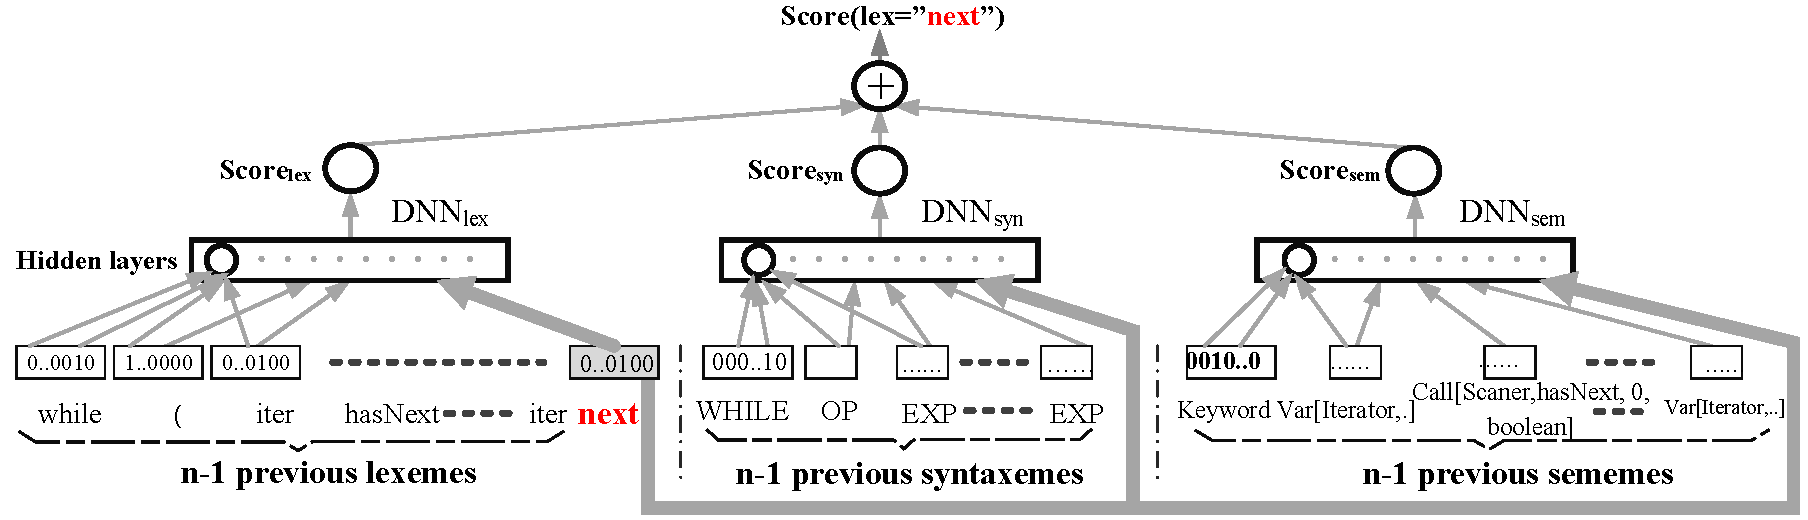
\includegraphics[width=6in]{contextmodel2.pdf} %contextmodel.pdf
\vspace{0.03in}
\caption{Context-aware DNN: Incorporating Syntactic and Type Contexts}
\label{contextfig}
\end{figure*}

\subsection{Overview and Key Ideas}
\label{keyideas}

%To achieve the goal of incorporating syntactic and semantic contexts,
%we design {\tool} with the following key ideas:

%Inspired by the success of DNN, 

We develop {\bf {\tool}}, a DNN-based LM for source
code, that 
%complements the local history of~$n$-gram by additionally
incorporates syntactic and type contexts (Fig.~\ref{contextfig}).
%We adapted Huang {\em et al.}~\cite{huang12}'s model for our new code
%features listed in Section~3:

%1. {\bf Syntaxeme and sememe sequences as contexts}. While the
%traditional DNN LM uses only $n$-1 prior lexical tokens (words),~we
%also attempt to parse the current file and derive the syntaxeme and
%sememe sequences for those tokens (if possible), and use those
%sequences as contexts. We expect that with more precise information on
%the current syntactic unit and on data/token types, DNN LM will be
%able to capture patterns at higher abstraction levels, thus, leading
%to more correct suggestion of the next token. For example,
%in Figure~\ref{contextfig}, with the token \code{hasNext} and the
%sememe \code{CALL [Scanner, hasNext, 0, boolean]} being in the
%contexts, {\tool} could rank the token \code{next} of \code{Scanner}
%higher in the output since \code{hasNext} of a \code{Scanner} object
%is often followed by a call to \code{next}. Instead of using only one
%DNN for the lexemes as in DNN LM, we input each lexeme and its syntax
%and semantic contexts into two additional DNNs
%(Figure~\ref{contextfig}), each of which is dedicated to incorporate
%one type of context.

%----------------------------------------------------------------------


1. {\bf Syntaxeme and sememe sequences as contexts}. While existing
deep learning LMs use only lexical code tokens with limited contexts,
we also attempt to parse the current file and derive the syntaxeme and
sememe sequences for those tokens (if possible), and use those
sequences as contexts. 

%We expect that with information on the current syntactic unit and
%data/token types, {\tool} is able to capture code patterns at higher
%abstraction levels.  For example, in Figure~\ref{contextfig}, with the
%token \code{hasNext} and the sememe \code{CALL [Scanner, hasNext, 0,
%    boolean]} being in the contexts, {\tool} could rank the token
%\code{next} of \code{Scanner} higher since \code{hasNext} of a
%\code{Scanner} object is often followed by a call to \code{next}, thus
%improving accuracy.


2. {\bf Multiple-prototype model (DNNs).} Instead of using only one
DNN for all sequences at three levels, we input each lexeme and its
syntax and type contexts into two additional DNNs, each of which is
dedicated to incorporate one type of context (See Fig.~\ref{contextfig}
for the model).
%
As shown in Huang {\em et al.}~\cite{huang12}, using a single DNN
would not capture well different meanings of the same lexeme (e.g.,
\code{next}) in different contexts (e.g., \code{LinkedList.next} or
\code{Scanner.next()}) as the model is influenced by all of them. They
showed that using multiple DNNs for multiple
representations in different contexts capture well a word in different
usages.
%When word meaning is still ambiguous given local context, we expect
%that information in other contexts can help disambiguation.
%\cite{huang12}.

3. {\bf Training objectives.}  There are following objectives in
training for {\tool}: 1) to train the first DNN to learn to determine
the potential next code token based on the $n$-1 {\em previous
  lexemes}, and 2) to train the two additional DNNs for contexts to
discriminate each correct next token $c$ from other tokens in the
vocabulary {\em given the window of $n$-1 previous lexemes} and {\em
  the syntactic/type contexts of that token $c$}. 
%
That is, the score should be large for the actual~next token, compared
to the score for other tokens.
%
Specifically, let us use $lex$ to denote the current sequence of $n$-1
prior lexemes. We aim to train {\tool} to discriminate the actual next
token $c$ (appearing~after $lex$) from the other tokens in the
vocabulary.
%
Let $Score_{syn}$ and $Score_{sem}$ be the scoring functions for two
DNNs  modeling syntactic and type contexts.  We aim
that with the input $lex$, they give the scores $Score_{syn}(c,syn)$
and $Score_{sem}(c,sem)$ for the correct token $c$ much higher than
the scores $Score_{syn}(c',syn)$ and $Score_{sem}(c',sem)$ for any
other token $c'$ in the vocabulary.
%
$syn$ and $sem$ are the sequences of $n$-1 prior syntaxemes and $n$-1
prior sememes representing the contexts for $c$ and $lex$. In
general, one can use any subsequences of the syntaxeme and sememe
sequences for the tokens from the beginning of a file to $c$ as
contexts.
%
However, performance will be an issue when the sequences are
long. Thus, we~used the same length ($n$-1) for syntaxeme and sememe
sequences.



As an example, we want to have the scores \code{$Score_{syn}$} and
\code{$Score_{sem}$} for the token \code{next} of \code{Scanner} to be
higher than the scores for other tokens. Mathematically, as 
in~\cite{huang12,collobert08}, we use a training objective
$O(c,syn)$ that minimizes the ranking loss for each pair of token $c$
and sequence $syn$ in a file, and gives the margin of 1 between two
such scores. Thus, for the sequence $lex$ ending with $c$, it is computed as in the following formula (1):
\[
O(c,syn) = \sum\limits_{c' \in V} max (0,1 - (Score_{syn}(c,syn) - Score_{syn}(c',syn)))
\]
If the margin between the two scores for $c$ and $c'$ is smaller than
1, the $2^{nd}$ argument in the $max$ function is greater than~0.  If
the margin is greater than 1, the $max$ function returns 0, helping
the objective $O$ reach its minimum.
%
Thus, by using the $max$ function, we aim to minimize that ranking
loss for $(c,syn)$.  The same training objectives $O(c,lex)$ and
$O(c,sem)$ are used for lexeme and sememe sequences.


\subsection{Model Architecture and Details}

\begin{figure}[t]
\centering
\includegraphics[width=3.2in]{msr17-dnn2.pdf} %dnn.pdf 0.47
\vspace{-0.06in}
\caption{Deep Neural Network Language Model for Source Code}
\label{dnnfig}
\end{figure}

Fig.~{\ref{dnnfig}} shows model architecture. It takes as input
3 levels of lexemes, syntaxemes, and sememes to
predict the next lexeme.
%
For training, for each sequence $s$ of length $n$, the correct lexeme
$c$ at the $n^{th}$ position of $s$ is fed into the input $lex_n$,
which is actually fed into three DNNs for three levels
(Fig.~\ref{contextfig}).
% Tien
%For training, the correct lexeme $c$ at the $n^{th}$ position of a
%sequence $s$ of length $n$ is fed into the input $lex_n$, which is fed
%into 3 DNNs at 3 levels as explained in Figure~\ref{contextfig}.
%
Three sequences of length $n$-1 for lexemes, syntaxemes, and sememes
corresponding to $s$ are fed into the other inputs.
%
For predicting, each candidate~$c$ in the lexeme vocabulary is fed
into the input $lex_n$ and $Score(c)$ is computed and normalized
(representing how likely $c$ is the next~token of the input~sequ\-ence
$lex_1, ..., lex_{n-1}$). All candidates are ranked via
their scores. 
%Details on training/predicting are given later.
The projection layer could be used in each DNN.

%lex_n = w_i

%score (lex_n = w_i) / sum (score (w_i))  (i from 1 to |V|)

%\vspace{0.03in}
\noindent {\bf Lexical level.} The input at this level is the
concatenated discrete feature vectors of $n$-1 prior lexemes $lex_1,
..., lex_{n-1}$ of the current $lex_n$.
%
Each lexeme is represented by a vector where only the index of that
lexeme is one.
%(all others are zeros). 
The role of projection for lexemes is for {\em word embedding}, i.e.,
to {\em map each lexeme to a continuous feature space} in the same manner in
Word2Vec~\cite{word2vec} (DNN LM also used projection):
%We expect that the ``related'' lexemes are mapped to nearby locations
%along some dimensions in that space:

${h_1}(y) = \tanh \left( {\sum\limits_{x = 1}^{|V|} {w_p(x,y)i(x)} +
  b_p(y)}\right),\forall y = 1, \cdots ,{M_1}$ 

%M_1=n-1

\noindent $i(x)$ is the value of node $x$ at the input; $h_1(y)$ is
the output value~of node $y$ in this projection layer; $w_p(x,y)$ is
the weight of the connection from input $x$ to output $y$, and
$b_p(y)$ is a bias value for node $y$; $M_1$ is the number of outputs
of this layer; and $V$ is the vocabulary.

%Mathematically, the formula (1) in Section~\ref{dnnbackgroundsec} is
%used but $p(y)$ is replaced by $h_1(y)$ and $M_p=M_1=n$-1. 

%($h_1(i)$ is the mapping from the input). 

Then, the output feature~vectors of this layer for $n$-1 prior lexemes
are concatenated with $lex_n$: $h_1 = [h_1(1);...; h_1(M_1);lex_n]$.
To compute the score of a node $y$ at the lexical level, we have:
\[\begin{array}{l}
{lex}(y) = \tanh \left( {\sum\limits_{x = 1}^{n} {w_{lex}(x,y){h_1}(x)} + b_{lex}(y) }\right),\forall y = 1, \cdots ,{M_{lex}}\\
Score_{lex} = \sum\limits_{y = 1}^{{M_{lex}}} {w'_{lex}(y){lex}(y) + b'_{lex}}  \quad \quad \quad \quad \quad \quad \quad \quad \quad \quad (2)
\end{array}\]
where $w_{lex}$ and $w'_{lex}$ are the weights at the lexical
level. $b_{lex}(y)$ and $b'_{lex}$ are the bias values for node $y$ here.

%\vspace{0.03in}
%\noindent {\bf Syntactic level.} For the score from the syntactic
%context DNN, we use the {\em sequence of $n$-1 syntaxemes} corresponding to
%the prior tokens, i.e., $n$-1 syntaxeme units \code{$syn_1$}, ...,
%\code{$syn_{n-1}$}.

\vspace{0.03in}
\noindent {\bf Syntactic level.} For the score from the DNN for syntactic
context, we use the {\em sequence of $n$-1 prior syntaxemes}
\code{$syn_1$}, ..., \code{$syn_{n-1}$} as context, assuming that $syn_n$ is the
syntaxeme for $lex_n$. A lexeme corresponds to only one syntaxeme, but
a syntaxeme can have multiple lexemes.
%
%Note that this is our design choice \#1. For the second, all
%syntaxemes for the tokens from the beginning of the file to the
%current position $n$ are used.
%
Each syntaxeme is represented by a vector where only the index of that
syntaxeme in the vocabulary is set to 1, while all others are 0s.
To form the syntactic context, we concatenate the vectors of $n$-1
syntaxemes with the vector of the lexical token $lex_n$ right
after the current lexical sequence $lex_1$, $lex_2$, ...,
$lex_{n-1}$. Thus, we have the combined vector $syn_h = [syn_1,
  syn_2,..., syn_{n-1}, lex_n]$. To compute the score for a node $y$
at the syntactic level, we use:
\[\begin{array}{l}
{syn}(y) = \tanh \left( {\sum\limits_{x = 1}^{n} {w_{syn}(x,y){syn_h}(x)} + b_{syn}(y) }\right),\forall y = 1,.,{M_{syn}}\\
Score_{syn} = \sum\limits_{y = 1}^{{M_{syn}}} {w'_{syn}(y){syn}(y) + b'_{syn}} \quad \quad \quad \quad \quad \quad \quad \quad \quad (3)
\end{array}\]
where $w_{syn}$ and $w'_{syn}$ are the weights at the syntactic
level. $b_{syn}(y)$ and $b'_{syn}$ are the bias values for a node $y$.
%at this level.

%here

During training, we will select a subset in the lexical vocabulary and
replace $lex_n$ with each of tokens in that subset to form multiple
combined vectors $syn_h$.
%several combined vectors will be formed by replacing
%$lex_n$ with several other words in the lexical vocabulary. 
The training objective is to minimize $O(lex_n,syn)$, i.e., the
ranking loss for each pair of token $lex_n$ and sequence $syn$
(Section~\ref{keyideas}). Note that, in formula~(1),
$Score_{syn}(c,syn)$ is equal to $Score_{syn}$ in formula~(3) where $c
= lex_n$ and $syn = [syn_1, ..., syn_{n-1}]$.

\vspace{0.03in}
\noindent {\bf Type level.} To compute the score from the DNN for
type context, we perform a similar process as the one at the
syntactic level, except that the syntaxemes are replaced by the
sememes of the current lexical sequence. That is, from the combined
vector for the type context, $sem_h = [sem_1, sem_2,...,
  sem_{n-1}, lex_n]$, we compute $sem(y)$ and $Score_{sem}$ as in
(3). The number of hidden nodes is $M_{sem}$. The weights will be
learned via training.
%
Similarly, the training objective is to minimize the ranking loss
$O(lex_n,sem)$ for each pair of token $lex_n$ and sequence
$sem$.


\vspace{0.02in}
\noindent {\bf Final score.} The~final score for a lexical token is
the normalized score of the sum of three scores over all~tokens.
%possible $w_i$ in~$V$.

%$Score$=$Score_{lex}$+$Score_{syn}$+$Score_{sem}$.

%The~final score for each lexical token $w_i$ is the sum of all of its
%scores at three levels:
%$Score$=$Score_{lex}$+$Score_{syn}$+$Score_{sem}$.
%----

%$Score$ at three levels and used for ranking in prediction.

%The scores are used to rank the tokens for prediction.

%---
%\vspace{0.03in}
%\noindent {\bf Semantic level.} To compute the score from the semantic
%context DNN, we perform a similar process as the one at the syntactic
%level, except that the syntaxemes are replaced by the sememes of the
%current lexical sequence. First, to form the semantic context, we
%concatenate the vectors of $n$-1 sememes with the vector of the next
%lexical token $lex_n$ right after the current lexical sequence. Thus,
%we have the combined vector $sem_h = [sem_1, sem_2,..., sem_{n-1},
%  lex_n]$. To compute the score for semantic context, we use a
%two-layer neural network as follows:
%\[\begin{array}{l}
%{sem}(y) = \tanh \left( {\sum\limits_{x = 1}^{n} {w_{sem}(x,y){sem_h}(x)} + b_{sem}(y) }\right),\forall y = 1, \%cdots ,{M_{sem}}\\
%Score_{sem} = \sum\limits_{x = 1}^{{M_{sem}}} {w'_{sem}(x,y){sem}(x) + b'_{sem}(y)} \quad (4)
%\end{array}\]
%$w_{sem}$ and $w'_{sem}$ are the weights at the semantic
%level. $b_{sem}(y)$ and $b'_{sem}(y)$ are biases at this level.
%Similarly, the training objective is to minimize the ranking loss
%$O(lex_n,sem)$ for sequences.
%------------

%Three output vectors of three input layers corresponding to lexical,
%semantic and syntactic levels will be concatenated and calculated by
%hidden layers of our model. The hidden layers can include many layers
%with different number of computation nodes at each layer. The task of
%each layer is to learn the link between syntactic, semantic and
%lexical at the corresponding abstraction level.

%The output of hidden layer will be used in output layer to estimate
%the probability that a lexical with index i in dictionary will appears
%at location n. The index i with high probability will be used to infer
%the corresponding lexeme at location n.




%The syntactic input layer takes representative vectors of $n-1$
%previous syntactic tokens.  Each syntactic token is the label
%syntactic role of corresponding lexical token. For examaple, syntactic
%tokens corresponding of \code{System . out . println (); } will be
%\code{MethodCall(System, . , out, . , prinln, ( , )), Term(;)}. The
%representative vectors are constructed similarly to those in lexical
%and semantic levels.

%The lexical input layer takes representative vectors of $n-1$ previous
%lexical tokens.  The representative vector of each token includes the
%value of 1 for element at index of the token's label in the
%dictionary. The other element will have value of 0. Hence, if the
%dictionary of all token's label has $V$ words, the representative
%vector will have 1 element of value 1 (at index of the token) and
%$V-1$ elements having value of 0.

%The semantic input layer takes representative vectors of $n-1$
%previous semantic tokens.  Each semantic token is the semantic
%annotation of corresponding lexical token in $n-1$ tokens.  For
%example, semantic annotation of tokens of \code{System . out . println
%  (); } will be \code{Type(System, System), Punc(.),
%  Field(OutputStream, out), Punc(.), MethodCall(void, println),
%  Punc((), Punc())}.  The representative vector of each token is
%constructed similarly to that for lexical token, i.e.  one element at
%dictionary index of the token have value of 1 and the others have
%value of 0.

%At input, our model will treat each level in the similar way. That is,
%the $n-1$ representative vectors of $n-1$ tokens will be concatenate
%with their sequential order. The combined vector (with length of
%$(n-1)V$) will be processed with the input layer $I$. The role of $I$
%is to projects the sparse vectors representing $n-1$ tokens to the
%corresponding vectors in continuous space. That step is important due
%to two reasons discussed in section {\ref{nnlmsec}}.

%\vspace{0.03in}

\subsection{Training and Predicting}

\noindent {\bf Training.}  We parse each file in the training
corpus to create lexeme, syntaxeme, and sememe sequences. We collect
all sequences of lexemes with a fixed length $n$: $[lex_1, lex_2,...,
  lex_n]$. The corresponding syntaxeme $syn_{n-1}$ and sememe
$sem_{n-1}$ of $lex_{n-1}$ are identified. We then collect $n$-1 prior
units of lexemes $lex=[lex_1, lex_2,..., lex_{n-1}]$, syntaxemes
$syn=[syn_1, syn_2,..., syn_{n-1}]$ and sememes $sem=[sem_1,
  sem_2,..., sem_{n-1}]$, and use them as input to {\tool} in
Fig.~\ref{dnnfig}. 

The token $lex_n$ is used as the correct next token and fed into the
input labeled $lex_n$. The score for that token is computed with the
current weights (weights are initialized in the beginning). Then,
{\tool} randomly selects a lexical token $c'$ (different from $lex_n$)
as a negative example for the pair $(lex_n,lex)$, and feeds it into
the input labeled $lex_n$ (instead of using the correct token
$lex_n$). The score $Score(c',lex)$ is computed. The difference of the
scores $Score(lex_n,lex)$ and $Score(c',lex)$ is recorded. Then, the
weights are updated for \code{DNN}$_{lex}$ to minimize the value of
the objective $O(lex_n,lex)$ (Section~\ref{keyideas}) by taking a
gradient step with respect to this choice $c'$. That is, we take the
derivative of the ranking loss with respect to the weights of the DNN.
%as in training for Huang's model~\cite{huang12}. 
{\tool} repeats the process for other token $c''$ in the lexeme
vocabulary until reaching a certain number of iterations. As suggested
in~\cite{huang12}, when there is sufficiently large number of
iterations, the quality is as good as using stochastic gradient
descent. The training process continues in the same way to train the
weights for the two other DNNs for syntaxemes and sememes except that
we use $Score(lex_n,syn)$ and $Score(lex_n,sem)$. Details on objective of minimizing ranking loss can be found
in~\cite{collobert08}.


%the other tokens $c'$ are used in place of $lex_n$ and their scores
%are computed. The weights will be adjusted to minimize the values of
%the objectives $O(lex_n,lex)$, $O(lex_n,syn)$, and $O(lex_n,sem)$ for
%each possible group of ($lex_n$, $lex$, $syn$, $sem$) found in the
%corpus.

%For efficient training, we followed the multi-objective joint training
%process by Collobert {\em et al.}~\cite{collobert08}. The process
%starts with the DNN for lexemes (\code{DNN}$_{lex}$). We randomly
%choose a lexical token $c'$ (differing from $lex_n$) as a negative
%example for each group ($c'$, $lex$, $syn$, $sem$). Then, the weights
%are updated for \code{DNN}$_{lex}$ via backpropagation by taking a
%gradient step with respect to this choice $c'$. That is, we take the
%derivative of the ranking loss with respect to the weights of the
%DNN. Next, the process repeats the same for the DNNs for syntaxemes
%and sememes. As suggested in~\cite{huang12}, we repeat it until reaching
%a certain number of iterations. More details are in~\cite{collobert08,huang12}.

%1. Select the next task.
%2. Select a random training example for this task.
%3. Update the NN for this task by taking a gradient
%step with respect to this example.
%4. Go to 1
%-------------------------

%For training, we follow the standard training procedure for deep
%neural network (DNN)~\cite{dnnbook} except for the pre-processing,
%computing the scores at three levels (see the above formulas), and the
%training objective. For the pre-processing, all the programs in the
%training corpus are processed to produce sequences of lexemes,
%syntaxemes, and sememes.  Each window of size $n$ ($n$-gram) is
%processed. The corresponding $n$-grams of syntaxemes and sememes are
%extracted. The $n$-1 elements of each of the lexeme, syntaxeme, and
%sememe sequences are used as the input for training. The scores for
%tokens are computed including for the last lexical token $c$ in the
%current $n$-gram. We use the ranking-loss training objective as
%in~\cite{collobert08}. That is, we aim to minimize the ranking loss
%$O$ for each sequence in the formula (2) (i.e., where the last token
%$c$ is replaced with others).

\vspace{0.02in}
\noindent {\bf Prediction.} At a point $L$ of suggestion in a program,
we process the code using PPA~\cite{ppa08} to construct the sequences
of syntaxemes and sememes up to $L$. For a fixed value of $n$, we
collect $n$-1 prior lexemes, syntaxemes, and sememes (from the last
token before $L$) and use them as the input of {\tool}. Then, each
token $c$ in the~vocabulary $V$ will be fed into the input labeled
$lex_n$ in Fig.~\ref{dnnfig}.~The score for $c$ is
computed and normalized to rank how likely the next token is $c$.
%All tokens in the lexical vocabulary are ranked based on their scores.




%\input{bayesmodel}
%\input{features}
\section{Empirical Evaluation}

%talk about other apps?

This section presents our empirical evaluation. In our experiments,
we aim 1) to evaluate {\tool}'s {\em accuracy} in two SE
applications: code completion and code migration; 2)
to compare it with the state-of-the-art approaches; and 3) to study
the impacts on accuracy of different {\em parameters} of the model and
those of {\em syntactic and semantic contexts}.

%next-token suggestion; 2) to compare {\tool} to the state-of-the-art
%LMs; 3) to study the impacts on accuracy of different {\em parameters}
%of the model and those of {\em syntactic and semantic contexts}; and
%4) to evaluate {\tool}'s accuracy in code~migration and code synthesis
%applications.

%$n$-gram LM and SLAMC~\cite{fse13}.



%Some projects are replaced if source code is not available anymore.

%We used the latest stable versions at the time of our experiments. 
%We also replaced some projects with new ones when the source code is
%not available anymore.

%\subsection{Data Collection}


% shows the statistics of our dataset. 

%It consists of 10 projects having more than 11,642 files, with 1.15M
%SLOCs and 8,987K $n$-grams with $n$=4. The last 3 columns show the
%sizes of the vocabularies of lexemes, syntaxemes, and sememes.


% Table generated by Excel2LaTeX from sheet 'systems'
\begin{table}[t]
  \centering
  \scriptsize
%footnotesize
%  \tabcolsep 3pt 
  \renewcommand{\arraystretch}{0.9}
  \caption{Subject Projects}
    \begin{tabular}{l|l|r|r|r|r|r|r}
    \hline
    Project & Rev & Files & KSLOCs & $n$-grams & $V_{lex}$   & $V_{syn}$  & $V_{sem}$ \\
    \hline
    ant   & 1.9.4 & 1,233 & 112.4 &        830,152  &    15,899  & 78    &      1,260  \\
    antlr & 3.5.1 & 276   & 40.3  &        264,640  &      5,534  & 77    &         538  \\
    batik & 1.7   & 1,447 & 152.8 &    1,174,800  &    21,709  & 76    &      1,590  \\
    cassandra & 2.1.2 & 960   & 190.9 &    1,450,201  &    18,601  & 78    &      1,330  \\
    db4o  & 7.2   & 1,722 & 83.6  &        620,229  &    10,381  & 75    &      1,249  \\
    itext & 5.3.5 & 503   & 69.3  &        612,571  &    11,648  & 77    &      1,158  \\
    jgit  & 2.3.0 & 1,011 & 101.8 &        858,799  &    13,494  & 78    &      1,295  \\
    lucene & 2.4.0 & 958   & 102.6 &        815,002  &    10,823  & 78    &      1,341  \\
    maven & 3.2.5 & 905   & 63.9  &        434,538  &      7,571  & 77    &      1,095  \\
    poi   & 3.8   & 2627  & 231.0 &    1,926,035  &    34,747  & 78    &      2,164  \\

    \hline
    \end{tabular}%
  \label{systemtab}%
\end{table}%



%\subsection{Featre Extraction}

%\input{features}

\subsection{Data Collection, Experimental Setting and Metrics}

%\section{Feature Extraction}

%We process all source files in every subject project. 

%We use 10-fold cross validation on each project. 
%We use the same setting as in the previous work on LM for source code.

To have the codebase for training, we collected several open-source
Java projects from SourceForge that have long histories and are
popularly used. For comparison, we selected the projects that were
used~in the state-of-the-art language model in~\cite{natural} (see Table
{\ref{systemtab}}).

We used the same procedure for evaluating the model's accuracy as in
the existing work~\cite{natural,tu-fse14,fse13}. 
Source files in a project are divided into 10 folds with equal numbers
of LOCs. One fold is used for testing and the others are used for
training. To study the impacts of features in a model, we integrated
the combinations of features and performed training and testing for
each newly built~model.

\noindent {\bf Training.} 
For each source file,
%in the training set, 
%we perform feature extraction. 
we use Eclipse for parsing and type analysis.
%%If a file is not compiled, we used PPA tool~\cite{ppa08} to perform
%%partial parsing as explained.
%PPA attempts to parse as many tokens as possible to build the abstract
%syntax tree (AST). 
%%PPA also performs semantic analysis including type resolution. 
Syntaxeme sequences are constructed according to the procedure
presented in Section~\ref{syntaxsec}.
% and Table~\ref{tab:javastruct}.
The sememe sequences are built from the result returned by Eclipse.
%The remaining unparseable code tokens are directly converted to their
%corresponding syntaxemes. 
If some tokens are unparseable or type information is not
available, the lexical tokens are annotated with the special
symbol \code{LEX}.
%
%Then, the unique tokens are collected into vocabularies at the three
%levels.  
For a pre-defined value of $n$, we collect into vocabularies and index
the $n$-grams of lexemes, syntaxemes, and sememes. For each lexical
token $lex_i$ in an $n$-gram, we build its {\em index vector} where
only the index of that token is set to 1.
% (Figure~\ref{dnnfig}).  
All the vectors for $lex_i$s
%each $n$-gram 
are concatenated. Similarly, we build the index vectors for the
syntaxeme and sememe sequences. Finally, the concatenated vectors are
used for~training.

\noindent {\bf Prediction.} 
For a source file in the testing set, our evaluation tool traverses
the sequence of its code sequentially. At each position of the
$i^{th}$ token, considering a fixed set of $n$-1 prior tokens, the
current language model is used to compute the top $k$ most likely code
tokens $c_1$, $c_2$, ..., $c_k$ for that position.
%the prior $n$-1 code tokens.
%
Since the previous tokens might not be complete, we used PPA
tool~\cite{ppa08} to perform partial parsing to produce the AST, and
semantic analysis for the code sequence $s$ from the starting of the
file to the current position.~From the AST and type information
returned from PPA, we build the sequences of syntaxemes
(Section~\ref{syntaxsec}) and sememes (Section~\ref{sememesec}). 
%The remaining unparseable code tokens are handled as special ones.
%
We then used the language model under investigation to suggest the
next token. If the actual token $s_i$ at position $i$ is among $k$
suggested tokens, we count this as a hit. The top-$k$ accuracy for
a code sequence is the ratio of the total hits over the total number
of suggestions. Total accuracy for a project is computed on all the
positions in its source files for the entire process.

%\subsubsection{Extracting Source Code Features}

%To extract those contextual features, we use a partial parser (\cite{}) to parse project's source code, 
%since the current editing code is not complete. The parser analyzes each project's source file to extract 
%sequential lexical tokens and abstract syntax tree (AST) of that file. The files' ASTs can be used to 
%extracted sequence of syntactic tokens corresponding to lexical tokens. The parser also uses semantic
%information to  determine the semantic tokens. The rules of determining syntactic and semantic sequence are
%determined in section {\ref{}}.

  %The output of our parsing process includes:

%1. All source files, with each file considered a document for Bayesian Model

%2. N-grams of lexical tokens extracted from the sequential lexical tokens of source files

%3. N-grams of syntactic tokens 

%4. N-grams of semantic tokens

%\subsubsection{Representing Features in DNN Model{\tool}}

%According to {\ref{}}, our model has three input levels. At each level, the sequence of $n-1$ tokens  (n-gram)
%is vectorized before used for calculation. In training, the model also considers the n-th token at predicting location.
%The model will use all input features to learn (in training step) the parameters of the model and use the features and
%learned parameters to predict next lexical tokens (in predicting step).

%Since the neural networks has input as concatenation of binary vectors representing tokens, our tool needs at first build representing binary vectors at then concatenate them. 

%The process of vectorization is:

%1. Build dictionaries of all unique tokens in lexical, syntactic and semantic levels. Let we assume the size of each 
%dictionary is $V_{lex}$, $V_{syn}$ and $V_{sem}$ correspondingly.

%2. For each lexical token $t$, we construct a vector $v_t$ of length $V_{lex}$. All elements of $v_t$ have value of $0$, 
%except the element at index $i_t$, where $i_t$ is the index of $t$ in lexical dictionary, has value of $1$.
%All vectors $v_1$, .. $v_{n-1}$ are concatenated and use by {\tool}.

%3. Similarly, we can construct the vectors for syntactic and semantic tokens.



%We implemented a tool which parse all source files from project to
%extract syntaxemes, sememes and lexemes. Given the lexemes of each
%source file, we evaluate the prediction of the lexeme at each
%location, given $n-1$ previous lexemes and the syntactic and semantic
%context.

%To evaluate our approach's accuracy and to compare it with other approach, we use the metrics of $top-k$ accuracy .....

\subsection{Accuracy With Different Contexts}

%  Table generated by Excel2LaTeX from sheet 'WithWithout'
\begin{table}[t]
  \centering
  \footnotesize
%  \tabcolsep 2pt
%  \small
  \caption{Accuracy With Different Contexts}
%(Lex+Syn+Sem={\tool})}
    \begin{tabular}{l|r|r|r|r|r|r}
    \hline
          & Top-1     & Top-2  & Top-3 & Top-4   & Top-5     & Top-10 \\
    \hline
    \code{Lex}         & 39.3\% & 53.4\% & 63.0\% & 67.2\% & 70.2\% & 77.2\%\\
    \code{Lex+Syn}     & 45.8\% & 59.7\% & 68.0\% & 72.0\% & 75.4\% & 82.5\%\\
    \code{Lex+Sem}     & 46.3\% & 61.5\% & 68.5\% & 72.5\% & 76.4\% & 82.6\%\\
    \code{{\bf Lex+Syn+Sem}} & {\bf 49.3}\% & {\bf 62.3}\% & {\bf 70.0}\% & {\bf 74.5}\% & {\bf 77.6}\% & {\bf 83.4}\%\\
    \hline
    \end{tabular}%
  \label{contextaccuracy}%
\end{table}%


%  Table generated by Excel2LaTeX from sheet 'WithWithout'
%\begin{table}[t]
%  \centering
%  \tabcolsep 2pt
%  \caption{Accuracy With Different Contexts}
%    \begin{tabular}{l|r|r|r|r|r|r}
%    \hline
%          & Top-1     & Top-2  & Top-3 & Top-4   & Top-5     & Top-10 \\
%    \hline
%    \code{Lex}         & 39.3\% & 53.4\% & 63.0\% & 67.2\% & 70.2\% & 77.2\%\\
%    \code{Lex+Syn}     & 45.8\% & 59.7\% & 68.0\% & 72.0\% & 75.4\% & 82.5\%\\
%    \code{Lex+Sem}     & 46.3\% & 61.5\% & 68.5\% & 72.5\% & 76.4\% & 82.6\%\\
%    \code{Lex+Syn+Sem} & 49.2\% & 62.3\% & 70.0\% & 74.5\% & 77.6\% & 83.4\%\\
%    \hline
%    \end{tabular}%
%  \label{contextaccuracy}%
%\end{table}%


In this experiment, we varied different context components in our
model and measured accuracy of newly configured
models. Table~\ref{contextaccuracy} shows the result. The first row is
for {\tool}~configured with only lexemes. This corresponds to the DNN
LM model in~\cite{DNNLM12}, but operates on lexemes. The second row is
for the model with both lexemes and syntaxemes. The third row is for
the model with both lexemes and sememes. The last row corresponds to
{\tool} model with all three types of features.
%We set the context's size $n$=4.

As seen, the models with contexts achieve better accuracy than the DNN
LM that treats source code as textual tokens and does not consider
syntactic and type contexts.

{\bf {\tool} with all three levels achieves even higher
accuracy} (last row). In comparison to the state-of-the-art DNN LM
(operating on lexemes), {\tool} has good relative improvement in
top-1 accuracy: 25.2\% (10\% absolutely).
%16.3\% (top-1) and 6.1\% (top-5). 
%
Importantly, it achieves high accuracy. In one out of two cases,
with a single suggestion, {\tool} correctly suggests the
next token. 
%In 3 out of 4 cases, the correct token is in the list of 4
%suggestions from {\tool}}. 
With~5 suggestions, it suggests the correct token in 77.6\% of the
cases.
%
%
With the addition of only syntaxemes, {\em the relative improvement in
top-1 accuracy (i.e., with a single suggestion) is 16.5\% (6.5\%
absolute improvement)}. 

%There is an interesting observation.  Despite that the context size
%$n$ is only 4 (which might not contain all syntaxemes of a syntactic
%unit, e.g., a \code{for} loop), {\tool} is still able to capture the
%beginning of a syntactic unit. For example, the syntaxemes \code{FOR}
%or \code{FORINIT} indicate the start of a \code{for} statement. The
%model uses it to sufficiently help predict the next token within the
%context defined by the unit.

%
%8.27%
%Examining the cases, we can see that with the syntaxemes as syntactic
%context, the lexical tokens relevant to surrounding ones are ranked
%higher because the grammar rules have restricted the valid syntactic
%units at a suggestion point. 
%Concrete examples are presented in Section~\ref{cases}.
%
%Moreover, 

Combining type context via sememes with lexemes improves
better than adding syntactic context via syntaxemes to lexemes
(i.e.,
\code{Lex+Sem} $>$ \code{Lex+Syn}). The model \code{Lex+Sem}
relatively improves 18.1\% at
%and 1.5\%
top-1 accuracy over the model \code{Lex}.
% and \code{Lex+Syn}, respectively.
%
After investigating, we found that data types and token types allow
\code{Lex+Sem} to rank the correct token at a suggestion point
higher than \code{Lex+Syn} with the syntactic context of surrounding
syntactic units. For example, pairs of API calls that often go
together (e.g., \code{Scanner.hasNext} and \code{Scanner.next}) are a
good foundation to suggest the second one if the first one is
encountered. In this case, \code{Lex+Syn} ranks multiple
identifiers (for method calls) higher than other types of
tokens, but \code{Scanner.next} is not the top one.

%After investigating, we found that data types and token types limit
%more the potentially valid tokens at a suggestion point than the
%syntactic context of current and containing syntactic units. In some
%suggestion cases, with syntactic context, the list of candidate tokens
%is in the tens of tokens. However, the sememes with data and token
%types can shorten that list to a few candidates. For example, pairs of
%method calls that often go together are a good indication for
%suggesting the second one if the first one is encountered.







%\subsection{Suggestion Accuracy}
\subsection{Accuracy Comparison to $n$-gram, SLAMC, DNN, RNN~LMs in Code Completion}

%Comparison to $n$-gram

%DNN LM without Context

%DNN LM with Context

%\subsubsection{Comparison to $n$-gram, SLAMC, DNN, RNN~LMs}

%This section presents our comparative evaluation to the
%state-of-the-art {\em statistical LM approaches}. 
We compare {\tool} with the $n$-gram LM used in Hindle {\em et
  al.}~\cite{natural}, Deep Neural Network LM (DNN LM)~\cite{DNNLM12},
Recurrent Neural Network LM (RNN LM)~\cite{mikolov10,white-msr15} used
in White {\em et al.}~\cite{white-msr15}, and Nguyen {\em et al.}'s
SLAMC~\cite{fse13}.
%
Note that the original DNN LM~\cite{DNNLM12} works on texts and RNN
LM~\cite{mikolov10} was applied on only lexical code tokens by White
{\em et al.}~\cite{white-msr15}.
%
However, in the previous experiment, we have shown that adding
syntaxemes and sememes improves over using only lexemes for DNN LM.
Thus, in this experiment, for DNN LM and RNN LM, we used as input all
three sequences of lexemes, syntaxemes, and sememes.
% by concatenating their vectors.
%we operate it by treating all code tokens as texts.
SLAMC~\cite{fse13} is a LM that works on the $n$-grams of sememes and
lexemes to predict the next lexical token (no syntactic information is
used). It explores the pairs of tokens that often go together to
improve its accuracy as well. 
%
It also integrates LDA~\cite{lda} to derive the {\em topics} of the
current file via Bayesian inference into a $n$-gram topic
model~\cite{fse13}.
%
%It also integrates the {\em topics} of the current file in the model
%via Bayesian inference. That is, it integrates topic modeling with
%$n$-gram into~a~$n$-gram topic model~\cite{fse13}.
%
%We did not compare our model to the one by Tu {\em et
%  al.}~\cite{tu-fse14}, which improves over $n$-gram with caching of
%entities' names, since SLAMC was shown to outperform that model with
%caching. 
We did not compare {\tool} to Raychev {\em et al.}~\cite{ethz-pldi14}
and GraLan~\cite{icse15} since they operate only on API elements.

%This section presents another experiment that we conducted to compare
%{\tool}'s accuracy to that of the state-of-the-art approaches. We
%compare it to $n$-gram LM by Hindle {\em et al.}~\cite{natural}, Deep
%Neural Network LM (DNN LM) (see Section~2), and SLAMC~\cite{fse13},
%our prior work on semantic LM. Note that the original DNN LM works on
%texts. However, in our experiment, we operate it by treating all code
%tokens as texts. SLAMC~\cite{fse13} is a LM that works on the
%$n$-grams of sememes and lexemes to predict the next lexical token (no
%syntactic information is used). It also explores the pairs of tokens
%that often go together to improve its accuracy. Importantly, SLAMC
%integrates the {\em topics} of the current file in the model via
%Bayesian inference. That is, it integrates topic modeling with
%$n$-gram into~a~$n$-gram topic model~\cite{fse13}.  We did not compare
%our model to the one by Tu {\em et al.}~\cite{tu-fse14}, which
%improves over $n$-gram with caching of entities' names, because SLAMC
%was shown to outperform that model with caching. We did not compare
%{\tool} to Raychev {\em et al.}~\cite{ethz-pldi14} and
%GraLan~\cite{icse15} since they operate only on API elements.

% Table generated by Excel2LaTeX from sheet 'summary (2)'
\begin{table}[t]
  \centering
 \footnotesize
 \tabcolsep 4.4pt
 \renewcommand{\arraystretch}{0.9}
  \caption{Accuracy Comparison on All Projects}
  \begin{tabular}{l|l|l|l|l|l|l}
    \hline
    \textbf{Project} & \textbf{Top} & \textbf{$n$-gram} & \textbf{SLAMC} & \textbf{DNN LM} & \textbf{RNN LM} & \textbf{{\tool}} \\
    \hline
    ant   & 1     & 45.7\% & 49.5\% & 51.3\% & 52.1\% & 54.3\% \\
          & 2     & 57.1\% & 60.3\% & 67.4\% & 64.8\% & 70.6\% \\
          & 5     & 63.6\% & 65.8\% & 78.5\% & 78.4\% & 83.7\% \\
    \hline
    antlr & 1     & 50.0\% & 53.0\% & 54.0\% & 52.4\% & 57.4\% \\
          & 2     & 61.6\% & 65.1\% & 69.0\% & 62.7\% & 70.3\% \\
          & 5     & 68.7\% & 70.8\% & 81.9\% & 72.5\% & 83.5\% \\
    \hline
    batik & 1     & 55.8\% & 59.0\% & 59.4\% & 61.1\% & 64.8\% \\
          & 2     & 69.3\% & 70.2\% & 74.6\% & 73.2\% & 78.5\% \\
          & 5     & 73.5\% & 73.7\% & 84.3\% & 84.0\% & 88.2\% \\
    \hline
    cassandra & 1 & 44.9\% & 48.2\% & 48.7\% & 51.4\% & 54.7\% \\
          & 2     & 53.7\% & 57.4\% & 63.8\% & 64.0\% & 66.7\% \\
          & 5     & 61.2\% & 64.0\% & 78.9\% & 79.7\% & 80.3\% \\
    \hline
    db4o  & 1     & 34.0\% & 38.7\% & 42.3\% & 44.1\% & 49.2\% \\
          & 2     & 41.7\% & 46.6\% & 56.4\% & 57.4\% & 62.3\% \\
          & 5     & 47.5\% & 50.1\% & 73.2\% & 73.1\% & 77.6\% \\
    \hline
    itext & 1     & 45.3\% & 48.7\% & 49.0\% & 51.1\% & 55.3\% \\
          & 2     & 60.3\% & 64.1\% & 64.4\% & 61.4\% & 68.0\% \\
          & 5     & 69.3\% & 72.1\% & 79.7\% & 70.9\% & 82.6\% \\
    \hline
    jgit  & 1     & 46.0\% & 49.0\% & 49.0\% & 56.4\% & 53.8\% \\
          & 2     & 60.9\% & 63.6\% & 64.4\% & 65.4\% & 68.0\% \\
          & 5     & 70.6\% & 72.2\% & 79.6\% & 73.7\% & 82.6\% \\
    \hline
     lucene & 1    & 48.0\% & 52.2\% & 53.0\% & 53.4\% & 57.2\% \\
          & 2     & 60.6\% & 63.5\% & 68.9\% & 69.1\% & 73.0\% \\
          & 5     & 71.6\% & 73.6\% & 82.6\% & 82.9\% & 85.2\% \\
    \hline
    maven & 1     & 39.1\% & 43.4\% & 43.1\% & 44.7\% & 47.6\% \\
          & 2     & 49.0\% & 52.7\% & 58.7\% & 56.5\% & 62.8\% \\
          & 5     & 54.9\% & 58.4\% & 71.9\% & 67.9\% & 75.2\% \\
    \hline
    poi   & 1     & 38.6\% & 42.4\% & 44.8\% & 43.9\% & 49.3\% \\
          & 2     & 47.5\% & 51.4\% & 59.0\% & 52.9\% & 63.3\% \\
          & 5     & 55.6\% & 57.9\% & 73.2\% & 60.5\% & 77.4\% \\
    \hline
 \end{tabular}%
  \label{allaccuracytab}%
\end{table}%

% Table generated by Excel2LaTeX from sheet 'summary (2)'
%\begin{table}[t]
%  \centering
% \small
% \tabcolsep 3pt
% \renewcommand{\arraystretch}{0.9}
%  \caption{Accuracy Comparison on All Projects}
%  \begin{tabular}{l|l|l|l|l|l}
%    \hline
%    \textbf{Project} & \textbf{Top} & \textbf{$n$-gram} & \textbf{SLAMC} & \textbf{DNN LM} & \textbf{{\tool}} \\
%    \hline
%    ant   & 1     & 45.7\% & 49.5\% & 51.3\% & 54.3\% \\
%          & 2     & 57.1\% & 60.3\% & 67.4\% & 70.6\% \\
%          & 5     & 63.6\% & 65.8\% & 78.5\% & 83.7\% \\
%    \hline
%    antlr & 1     & 50.0\% & 53.0\% & 54.0\% & 57.4\% \\
%          & 2     & 61.6\% & 65.1\% & 69.0\% & 70.3\% \\
%          & 5     & 68.7\% & 70.8\% & 81.9\% & 83.5\% \\
%    \hline
%    batik & 1     & 55.8\% & 59.0\% & 59.4\% & 64.8\% \\
%          & 2     & 69.3\% & 70.2\% & 74.6\% & 78.5\% \\
%          & 5     & 73.5\% & 73.7\% & 84.3\% & 88.2\% \\
%    \hline
%    cassandra & 1     & 44.9\% & 48.2\% & 48.7\% & 54.7\% \\
%          & 2     & 53.7\% & 57.4\% & 63.8\% & 66.7\% \\
%          & 5     & 61.2\% & 64.0\% & 78.9\% & 80.3\% \\
%    \hline
%    db4o  & 1     & 34.0\% & 38.7\% & 42.3\% & 49.2\% \\
%          & 2     & 41.7\% & 46.6\% & 56.4\% & 62.3\% \\
%          & 5     & 47.5\% & 50.1\% & 73.2\% & 77.6\% \\
%    \hline
%    itext & 1     & 45.3\% & 48.7\% & 49.0\% & 55.3\% \\
%          & 2     & 60.3\% & 64.1\% & 64.4\% & 68.0\% \\
%          & 5     & 69.3\% & 72.1\% & 79.7\% & 82.6\% \\
%    \hline
%    jgit  & 1     & 46.0\% & 49.0\% & 49.0\% & 53.8\% \\
%          & 2     & 60.9\% & 63.6\% & 64.4\% & 68.0\% \\
%          & 5     & 70.6\% & 72.2\% & 79.6\% & 82.6\% \\
%    \hline
%    lucene & 1     & 48.0\% & 52.2\% & 53.0\% & 57.2\% \\
%          & 2     & 60.6\% & 63.5\% & 68.9\% & 73.0\% \\
%          & 5     & 71.6\% & 73.6\% & 82.6\% & 85.2\% \\
%    \hline
%    maven & 1     & 39.1\% & 43.4\% & 43.1\% & 47.6\% \\
%          & 2     & 49.0\% & 52.7\% & 58.7\% & 62.8\% \\
%          & 5     & 54.9\% & 58.4\% & 71.9\% & 75.2\% \\
%    \hline
%    poi   & 1     & 38.6\% & 42.4\% & 44.8\% & 49.3\% \\
%          & 2     & 47.5\% & 51.4\% & 59.0\% & 63.3\% \\
%          & 5     & 55.6\% & 57.9\% & 73.2\% & 77.4\% \\
%    \hline
% \end{tabular}%
%  \label{allaccuracytab}%
%\end{table}%

%% Table generated by Excel2LaTeX from sheet 'summary'
%\begin{table}[t]
%  \centering
%  \tabcolsep 3pt
%  \caption{Accuracy Comparison of Different Models}
%    \begin{tabular}{l|l|l|l|l|l}
%    \hline
%    \textbf{System} & \textbf{Top} & \textbf{\tool}* & \textbf{\tool} & \textbf{N-gram} & \textbf{SLAMC} & \textbf{SLAMC+Syn} \\
%    \hline
%    ant   & 1     & 51.3\% & 54.3\% & 45.7\% & 49.5\% & 51.3\% \\
%          & 2     & 67.4\% & 70.6\% & 57.1\% & 60.3\% & 62.5\% \\
%          & 5     & 78.5\% & 83.7\% & 63.6\% & 65.8\% & 67.9\% \\
%		\hline    			
%    antlr & 1     & 54.0\% & 57.4\% & 50.0\% & 53.0\% & 55.6\% \\
%          & 2     & 69.0\% & 70.3\% & 61.6\% & 65.1\% & 66.4\% \\
%          & 5     & 81.9\% & 83.5\% & 68.7\% & 70.8\% & 72.1\% \\
%		\hline
%    batik & 1     & 59.4\% & 64.8\% & 55.8\% & 59.0\% & 61.5\% \\
%          & 2     & 74.6\% & 78.5\% & 69.3\% & 70.2\% & 71.3\% \\
%          & 5     & 84.3\% & 88.2\% & 73.5\% & 73.7\% & 74.8\% \\
%		\hline			
%    cassandra & 1     & 48.7\% & 54.7\% & 44.9\% & 48.2\% & 50.8\% \\
%          & 2     & 63.8\% & 66.7\% & 53.7\% & 57.4\% & 59.1\% \\
%          & 5     & 78.9\% & 80.3\% & 61.2\% & 64.0\% & 65.3\% \\
%		\hline			
%    db4o  & 1     & 42.3\% & 48.8\% & 34.0\% & 38.7\% & 41.0\% \\
%          & 2     & 56.4\% & 61.5\% & 41.7\% & 46.6\% & 48.7\% \\
%          & 5     & 73.2\% & 76.9\% & 47.5\% & 50.1\% & 52.1\% \\
%		\hline			
%    itext & 1     & 49.0\% & 55.3\% & 45.3\% & 48.7\% & 52.5\% \\
%          & 2     & 64.4\% & 68.0\% & 60.3\% & 64.1\% & 66.6\% \\
%          & 5     & 79.7\% & 82.6\% & 69.3\% & 72.1\% & 73.7\% \\
%		\hline			
%    jgit  & 1     & 49.0\% & 53.8\% & 46.0\% & 49.0\% & 51.1\% \\
%          & 2     & 64.4\% & 68.0\% & 60.9\% & 63.6\% & 64.7\% \\
%          & 5     & 79.6\% & 82.6\% & 70.6\% & 72.2\% & 73.3\% \\
%		\hline			
%    lucene & 1     & 53.0\% & 57.2\% & 48.0\% & 52.2\% & 54.4\% \\
%          & 2     & 68.9\% & 73.0\% & 62.6\% & 63.5\% & 65.6\% \\
%          & 5     & 82.6\% & 85.2\% & 71.6\% & 73.6\% & 75.5\% \\
%		\hline			
%    maven & 1     & 43.1\% & 47.6\% & 39.1\% & 43.4\% & 45.0\% \\
%          & 2     & 58.7\% & 62.8\% & 49.0\% & 52.7\% & 54.3\% \\
%          & 5     & 71.9\% & 75.2\% & 54.9\% & 58.4\% & 60.0\% \\
%		\hline			
%    poi   & 1     & 44.8\% & 49.3\% & 38.6\% & 42.4\% & 44.3\% \\
%          & 2     & 59.0\% & 63.3\% & 47.5\% & 51.4\% & 53.4\% \\
%          & 5     & 73.2\% & 77.4\% & 55.6\% & 57.9\% & 59.4\% \\
%    \hline
%    \end{tabular}%
%  \label{allaccuracytab}%
%\end{table}%


\begin{figure}[t]
\centering
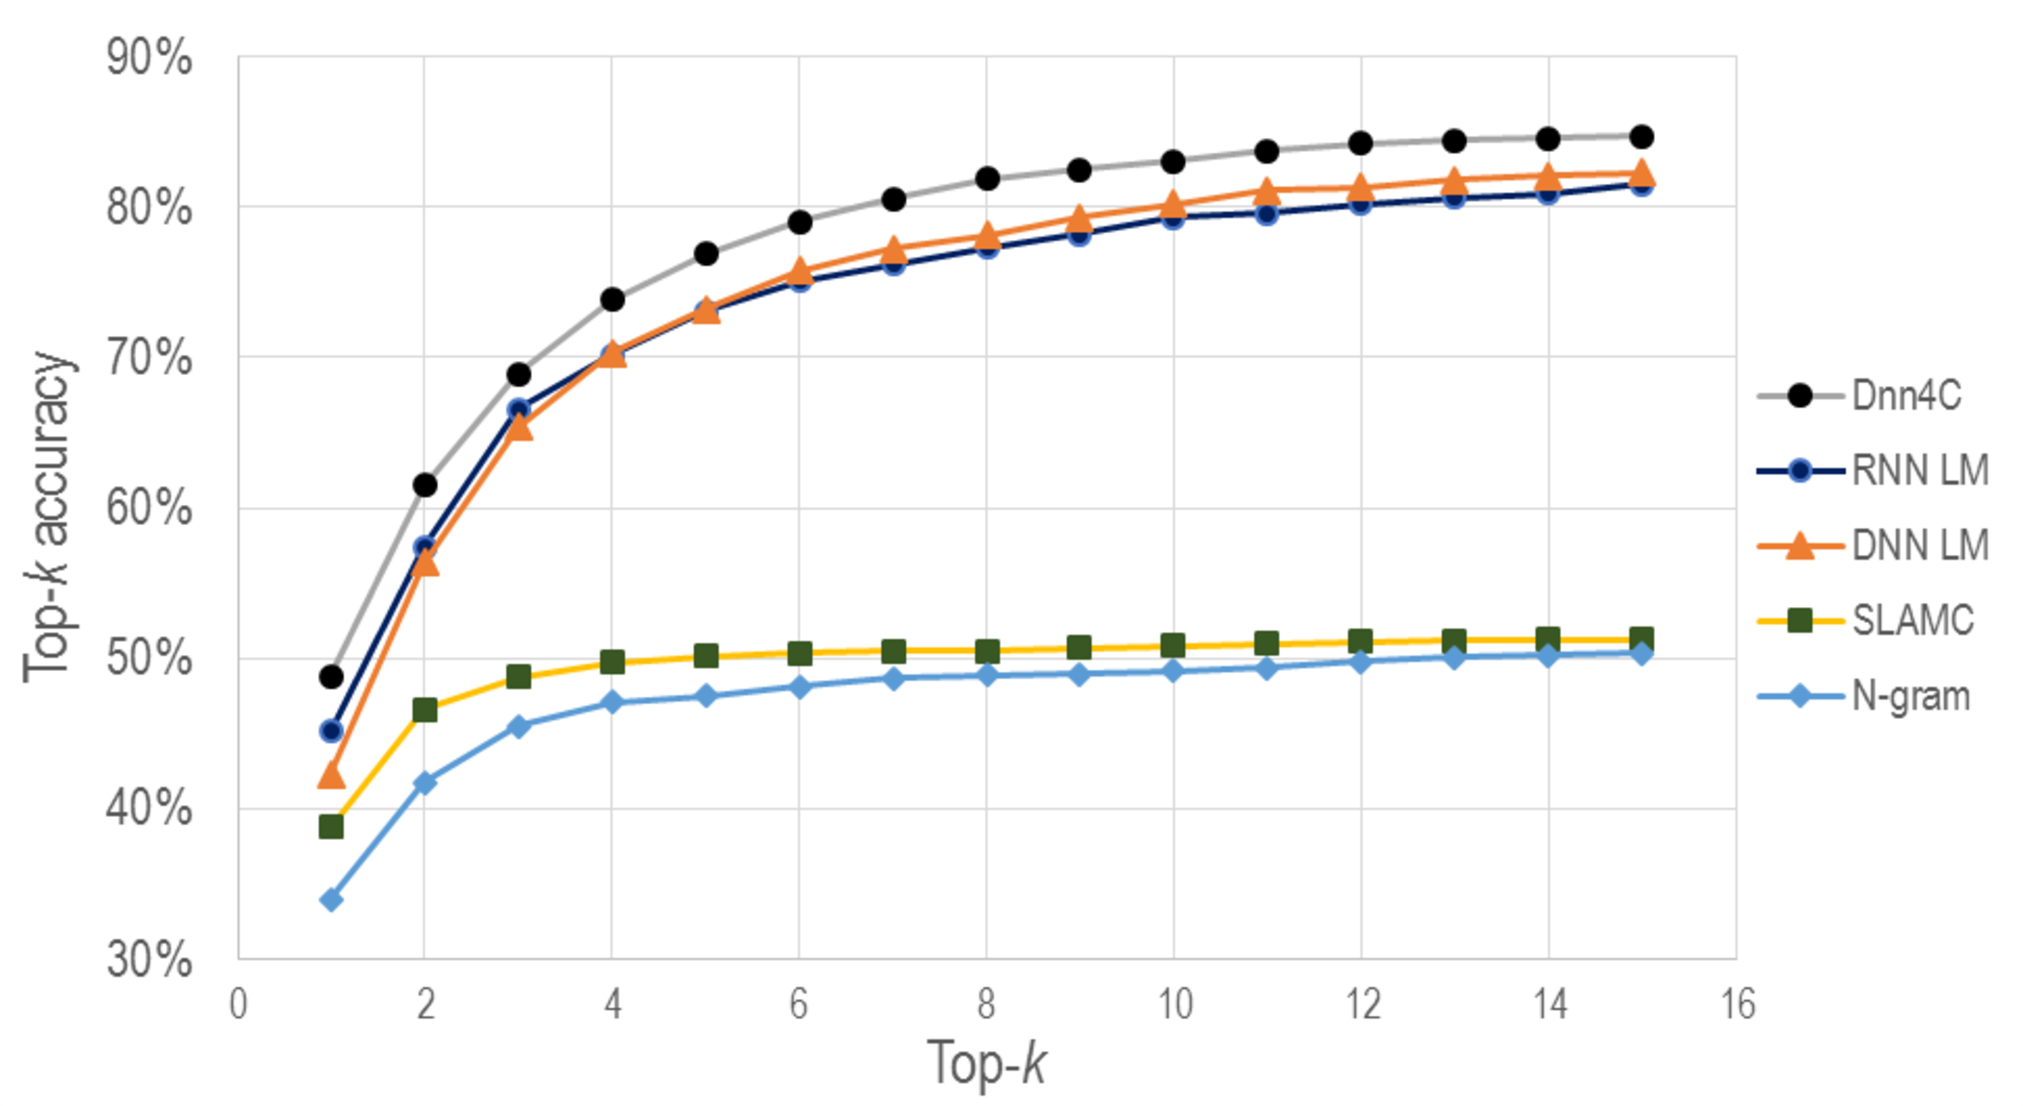
\includegraphics[width=3.5in]{db4o-new-3.pdf} %db4o-new-2.pdf {0.5 db4o.pdf, 0.46 sensitivity_approaches.pdf}
\vspace{-0.05in}
\caption{Top-$k$ Accuracy of Different Approaches on Db4o}
\label{approachesfig}
\end{figure}

%
%In general, {\tool} achieves higher accuracy than other approaches
%including DNN LM. {\tool} and DNN LM, which are based on DNN, achieve
%much higher accuracy than others in the larger values of top rank $k$,
%and reasonably higher accuracy in the smaller values of $k$.
%

Fig.~\ref{approachesfig} shows the comparison on \code{Db4o}
project for top-$k$~accuracy, $k$ = 1--15.  As seen,
{\tool} achieves higher~accuracy than the other approaches. At top-1
accuracy, {\tool} has relative improvements of {\bf 11.6\%}, {\bf
  16.3\%, 27.1\%}, and {\bf 44.7\%} over RNN LM, DNN LM, SLAMC, and
$n$-gram models, respectively. 
%
%At top-5 accuracy, such improvements are {\bf 6.2\%}, {\bf 6\%}, {\bf
%  54.9\%}, and {\bf 63.4\%}.
%
The three NN-based models achieve higher accuracy than the two
$n$-gram-based ones.
%, SLAMC and $n$-gram LM. 
%
%Such comparison was reported for texts in NLP~\cite{dnnbook}.
%
%This result confirms such comparison for source code. 
Among the NN-based models, with the same three features, {\tool}
outperforms RNN LM and DNN LM~relatively {\bf 11.6\%} and {\bf 16.3\%}
at top-1 accuracy. The absolute improvement percentages are reported
in Table~\ref{allaccuracytab}.
At a higher top rank $k$ from 10--15, {\tool} has much higher accuracy
than $n$-gram ({\bf 68.9\%} relatively) and SLAMC ({\bf 66.0\%}), and
higher than both RNN and DNN LMs.

% ({\bf 3.5\%}, {\bf 3.8\%}).

%Moreover, {\tool} outperforms DNN LM from 2.8--15.3\% for all top
%ranks $k$.

Table~\ref{allaccuracytab} shows the comparison result for {\em all
  projects}. At top-1 accuracy, {\tool} achieves relative improvements
from {\bf 14.8--44.7\%} over $n$-gram, {\bf 8.3--27.1\%} over SLAMC,
{\bf 5.9--16.3\%} over DNN LM, and {\bf 5.6--11.6\%} over RNN LM.

% ICSE'16
%If the models would suggest 5 candidates for the next token, {\tool}
%achieves relatively higher accuracy from {\bf 17.0--61.9\%} over
%$n$-gram model, from {\bf 14.4--53.5\%} over SLAMC, and from {\bf
%  1.8--6.7\%} over DNN LM. 
%


% in code suggestion than DNN LM, SLAMC, and $n$-gram models.


%Table {\ref{allaccuracytab}} shows the accuracy of our approach compared with other approaches. Column {\textbf{\tool}} is corresponding to our approach. Column {\textbf{\tool}*} is the accuracy of our tool without consideration of syntactic and semantic information.  Column {\textbf{N-gram}} is for N-gram approach,  column {\textbf{SLAMC}} is for SLAMC model modified to recommend lexeme and column {\textbf{SLAMC+Syn}} is the accuracy with SLAMC model extended with syntactic features.

%Implication:

%Tien
%1. {\textbf{\tool}} always achieve the best results in comparison with
%other approaches. {\textbf{\tool}*} achieve better results than
%{\textbf{N-gram}} and {\textbf{SLAMC}}. Its accuracy is comparable to
%{\textbf{SLAMC+Syn}} at low $k$ ( in $top-k$) but better than
%{\textbf{SLAMC+Syn}} at high $k$. {\textbf{SLAMC+Syn}} achieve better
%accuracy than {\textbf{N-gram}} and {\textbf{SLAMC}} but less accuracy
%than {\textbf{\tool}}.

%2. In details, at $top-1$, {\textbf{\tool}*} has better accuracy than
%{\textbf{N-gram}} from 3.0\% to 8.3\% (6.5\% to 24.4\% relatively).
%It improves over {\textbf{SLAMC}} from 0.0\% to 3.6\% (0.0\% to 9.3\%
%relatively). In some cases, {\textbf{\tool}*}'s accuracy is higher
%than {\textbf{SLAMC+Syn}} and in other cases, it is not. However, the
%difference is not significant.  {\textbf{\tool}} improves over
%{\textbf{N-gram}} from 7.4\% to 14.8\% (14.8\% to 43.5\% relatively).
%It improves over {\textbf{SLAMC+Syn}} from 1.8\% to 7.8\% (3.2\% to
%19.0\% relatively).


%3. At $top-5$, {\textbf{\tool}*} has better accuracy than
%{\textbf{N-gram}} from 9.0\% to 25.7\% (12.7\% to 54.1\% relatively).
%It improves over {\textbf{SLAMC}} from 7.4\% to 23.1\% (10.2\% to
%46.1\% relatively). It also improves over {\textbf{SLAMC+Syn}} from
%6.0\% to 21.1\% (8.1\% to 40.5\% relatively).  {\textbf{\tool}}
%improves over {\textbf{N-gram}} from 12.0\% to 29.4\% (17.0\% to
%61.9\% relatively).  {\textbf{\tool}} improves over
%{\textbf{SLAMC+Syn}} from 8.9\% to 24.8\% (12.1\% to 47.6\%
%relatively).  We checked the reason that {\textbf{\tool}} and
%{\textbf{\tool}*} have much improvement at high $top-k$. We saw that
%{\textbf{N-gram}}, {\textbf{SLAMC}} and {\textbf{SLAMC+Syn}} cannot
%predict $n-gram$ if that $n-gram$ has never appeared which leads to
%the $top-k$ accuracy get flat at high $k$. In other way,
%{\textbf{\tool}*} and {\textbf{\tool}} can predict event $n-gram$
%which has never appeared due to the mechanism of similar context in
%DNN language model.

%\[MRR({T_{test}},{T_{pred}}) = \frac{1}{{|{T_{test}}|}}\sum\limits_{i = 1}^{|{T_{test}}|} {\frac{1}{{index_i}}} \]

% Table generated by Excel2LaTeX from sheet 'summary'
\begin{table}[t]
  \centering
  \small
  \tabcolsep 3pt 
  \renewcommand{\arraystretch}{0.7}
  \caption{Mean Reciprocal Rank (MRR) Comparison}
    \begin{tabular}{l|l|l|l|l|l}
    \hline
    \textbf{Project} & {\textbf{$N$-gram}} & {\textbf{SLAMC}} & \textbf{DNN LM} & {\bf RNN LM} & \textbf{{\tool}} \\
    \hline
    ant   & 0.537 & 0.568 & 0.639 &     0.639   & 0.662 \\
    antlr & 0.584 & 0.616 & 0.662 &     0.628   & 0.695 \\
    batik & 0.640 & 0.674 & 0.706 &     0.719   & 0.737 \\
    cassandra & 0.519 & 0.555 & 0.616 & 0.638   & 0.656 \\
    db4o  & 0.400 & 0.439 & 0.581 &     0.586   & 0.611 \\
    itext & 0.577 & 0.617 & 0.625 &     0.601   & 0.656 \\
    jgit  & 0.588 & 0.619 & 0.673 &     0.647   & 0.701 \\
    lucene & 0.599 & 0.631 & 0.689 &    0.681   & 0.713 \\
    maven & 0.463 & 0.524 & 0.558 &     0.553   & 0.578 \\
    poi   & 0.459 & 0.492 &  0.563 &    0.516  & 0.583 \\
    \hline
    \end{tabular}
  \label{mrrtab}%
\end{table}%

% Table generated by Excel2LaTeX from sheet 'summary'
%\begin{table}[t]
%  \centering
%	\tabcolsep 3pt 
%  \renewcommand{\arraystretch}{0.7}
%  \caption{Mean Reciprocal Rank (MRR) Comparison}
%    \begin{tabular}{l|l|l|l|l}
%    \hline
%    \textbf{Project} & {\textbf{$N$-gram}} & {\textbf{SLAMC}} & \textbf{DNN LM} & \textbf{{\tool}} \\
%    \hline
%    ant   & 0.537 & 0.568 & 0.639 & 0.662 \\
%    antlr & 0.584 & 0.616 & 0.662 & 0.695 \\
%    batik & 0.640 & 0.674 & 0.706 & 0.737 \\
%    cassandra & 0.519 & 0.555 & 0.616 & 0.656 \\
%    db4o  & 0.400 & 0.439 & 0.581 & 0.611 \\
%    itext & 0.577 & 0.617 & 0.625 & 0.656 \\
%    jgit  & 0.588 & 0.619 & 0.673 & 0.701 \\
%    lucene & 0.599 & 0.631 & 0.689 & 0.713 \\
%    maven & 0.463 & 0.524 & 0.558 & 0.578 \\
%    poi   & 0.459 & 0.492 &  0.563 & 0.583 \\
%    \hline
%    \end{tabular}
%  \label{mrrtab}%
%\end{table}%


\vspace{0.03in}
\noindent {\bf Mean Reciprocal Rank (MRR).} We also
measured Mean Reciprocal Rank (MRR) to evaluate the models based on the
ranked list of suggested tokens.
%
The MRR value is computed as the average of the reciprocal ranks of
results for a set of suggestion cases:
\indent $MRR = \frac{1}{{|{T_{test}}|}}\sum\limits_{i = 1}^{|{T_{test}}|} {\frac{1}{{index_i}}} $
where $index_i$ is the index of the actual token in the
resulting ranked list at the $i$-th suggestion, and $|T_{test}|$ is
the number of suggestion cases.
%
%where $T_{test}$ is the true next tokens in the testing set for
%suggestion; $index_i$ is the index in the ranked list of predicted
%token at a suggestion, where the true next token is retrieved for the
%$i$-th query in the testing set. 
The closer to 1 the MRR value, the better the ranking of a model. 

As seen in Table~\ref{mrrtab}, {\tool} can achieve the highest MRR of
0.737, meaning that {\em on average in 2 suggestion cases, it can
  correctly rank the actual token as the top candidate in one case and
  at the second place in the resulting list in the other case}. For
all projects, MRR is 0.66 on average. That is, {\em among 3 cases, it
  would rank the actual token at the second place in two cases, and
  likely rank the actual token as the top candidate in the other
  case}.

In comparison, {\tool} improves MRR,
% relatively over the $n$-gram model up to {\bf 52.6\%}, over SLAMC up
% to {\bf 39.1\%}, over DNN LM up to {\bf 6.4\%}, and over RNN LM up
% to {\bf 13.0\%}.
\ie for a suggestion, the actual next token is generally ranked
higher in {\tool}'s resulting list than in the resulting lists of
other approaches.

%%In brief, {\em {\tool} consistently achieves better accuracy than others}.

%In comparison, {\tool} improves MRR accuracy relatively over the
%$n$-gram model from {\bf 13.7--52.6\%}, the SLAMC model from {\bf
%  9.3--39.1\%}, the DNN LM from {\bf 3.5--6.4\%}, the RNN LM from {\bf
%  2.7--5.5\%}.
%---------------------------

%This result is consistent with the comparison using top-$k$ accuracy.

%Moreover, in the subject project \code{batik}, with the MRR of {\bf
%  0.737}, every time that {\tool} has ranked the actual next token at
%the second place in its resulting list, it would likely rank the
%actual token as the top candidate for the next suggestion. On average,
%after every two times of ranking for the actual token at the second
%place, {\tool} would rank the actual token at the top.

%-------
%As seen in Table~\ref{mrrtab}, {\tool} improves MRR accuracy
%relatively over the $n$-gram model from {\bf 13.7--52.6\%}, the SLAMC
%model from {\bf 9.3--39.1\%}, and the DNN LM from {\bf 3.5--6.4\%}.
%
%That is, for a suggestion, the actual next token is generally ranked
%higher in {\tool}'s resulting list than the resulting lists of other
%models.  This result is consistent with the comparison using
%top-$k$ accuracy.
%
%Moreover, in the subject project \code{batik}, with the MRR of {\bf
%  0.737}, every time that {\tool} has ranked the actual next token at
%the second place in its resulting list, it would likely rank the
%actual token as the top candidate for the next suggestion. On average,
%after every two times of ranking for the actual token at the second
%place, {\tool} would rank the actual token at the top.
%------

%That is, with its suggestion list, {\tool} achieves higher accuracy in
%suggesting the next token.


%Those ranked lists of links $L_{pred}$ are used to evaluate a goal
%function \code{MAP($G_{test}, L_{pred}$)}, which is used to find the
%optimized value of $\alpha_1$.
%The $\alpha_1$ value corresponding to the highest value for \code{MAP}
%will be returned. The goal function $MAP$ in our algorithm is the mean
%average precision as proposed in {\cite{sun-ase11}}.










%4. To see if there are significant improvement over different approach, We then use t-test (with confidence of 0.95) over the $top-k$ accuracy to check the significance of hypotheses that an approach has more significant improvement over other approach. A hypothesis is considered significant if checking $p-value$ is smaller than 0.005.
%% Table generated by Excel2LaTeX from sheet 'summary'
%\begin{table}[h]
  %\small
	%\tabcolsep 1pt
  %\centering
    %\begin{tabular}{l|l|l|l|l}
    %\hline
           %&{\textbf{N-gram}}<{\textbf{SLAMC}} & {\textbf{SLAMC}}<{\textbf{SLAMC+Syn}} & {\textbf{SLAMC+Syn}}<{\textbf{\tool}} & {\textbf{\tool}}<{\textbf{\tool}*} \\
    %\hline
    %p-value&$10^{-14}$     & $10^{-16}$          & $0.0005$         & $10^{-15}$ \\
    %\hline
    %\end{tabular}%
  %\label{testingtab}%
  %\caption{Testing Significant Improvement between Approaches}
%\end{table}%
%
%Table {\ref{testingtab}} shows that our approaches are better than approaches based on {\textbf{SLAMC}}, which in turn better than {\textbf{N-gram}} approach.
%
%\subsection{Case Studies}


%%%% REMOVED
%\input{bayesmodel}


%\subsection{Sensitivity Analysis}
\subsection{Impacts of Factors on Accuracy}

We evaluate the impact of different factors and parameters of {\tool}
on its code completion accuracy. We chose Db4o, one of the largest
subject systems for this study.






%previous work [25] shows that DNN-based model can capture the global
%context from distant tokens. Moreover, Table_4 and the works [27,39]
%showed that expanding the window more than 5 tokens does not improve
%accuracy much, but significantly increases running time.

\input{saner18-size-context}

\input{saner18-hidden}

%This~shows very high accuracy of {\tool} using DNN with
%syntactic/semantic contexts.
%This result shows the benefits of using deep learning with
%incorporating syntactic and semantic contexts in code suggestion.


%\begin{figure}[t]
%\centering
%\includegraphics[width=0.46\textwidth]{sensitivity_combinations.pdf}
%\caption{Top-k Accuracy with and without Syntactic and Semantic Context}
%\label{combinationfig}
%\end{figure}

%We checked the accuracy of our approach with/without syntactic and semantic 
%context compared with {\textbf{N-gram}} and {{\textbf{SLAMC}}.

%Figure {\ref{approachesfig}} shows $top-k$ accuracy of different
%approaches.  As seen, {\textbf{\tool}*} achieves higher accuracy than
%{\textbf{\tool}} especially at top 1. It suggests that our model of
%integrating syntactic and semantic context using deep learning works
%well.


%DNN 

%DNN + syntax

%DNN + sememe

%DNN + syntax + sememe  = DNN4C




% Table generated by Excel2LaTeX from sheet 'WithWithout'
%\begin{table}[t]
%  \centering
%  \tabcolsep 2pt
%  \caption{Accuracy With Different Contexts}
%    \begin{tabular}{l|r|r|r|r|r|r|r}
%    \hline
%          & Top-1     & Top-2  & Top-3 & Top-4   & Top-5     & Top-10    & Top-20 \\
%    \hline
%    \code{Lex}         & 42.3\% & 56.4\% & 66.0\% & 70.2\% & 73.2\% & 80.2\% & 83.0\% \\
%    \code{Lex+Syn}     & 45.8\% & 59.7\% & 68.0\% & 72.0\% & 75.4\% & 82.5\% & 85.1\% \\
%    \code{Lex+Sem}     & 48.4\% & 61.5\% & 68.5\% & 73.0\% & 76.8\% & 82.6\% & 85.3\% \\
%    \code{Lex+Syn+Sem} & 49.2\% & 62.3\% & 70.0\% & 74.5\% & 77.6\% & 83.4\% & 85.6\% \\
%    \hline
%    \end{tabular}%
%  \label{contextaccuracy}%
%\end{table}%


%\begin{table}[t]
%  \centering
%  \tabcolsep 2pt
%  \caption{Accuracy With Different Contexts}
%    \begin{tabular}{l|r|r|r|r|r|r|r}
%    \hline
%          & Top-1     & Top-2  & Top-3 & Top-4   & Top-5     & Top-10    & Top-20 \\
%    \hline
%    \code{Lex}         & 39.3\% & 53.4\% & 63.0\% & 67.2\% & 70.2\% & 77.2\% & 80.0\% \\
%    \code{Lex+Syn}     & 45.8\% & 59.7\% & 68.0\% & 72.0\% & 75.4\% & 82.5\% & 85.1\% \\
%    \code{Lex+Sem}     & 48.4\% & 61.5\% & 68.5\% & 73.0\% & 76.8\% & 82.6\% & 85.3\% \\
%    \code{Lex+Syn+Sem} & 49.2\% & 62.3\% & 70.0\% & 74.5\% & 77.6\% & 83.4\% & 85.6\% \\
%    \hline
%    \end{tabular}%
%  \label{contextaccuracy}%
%\end{table}%



%\input{bayesmodel}

\subsection{Application of {\tool} in Code Migration}

We conducted another experiment to show a useful application of our
model in code migration. We used {\tool} as a language model in a
phrase-based statistical machine translation tool,
Phrasal~\cite{phrasal10}, to {\em take a method in Java and produce a
  respective method in C\texttt{\#}}. Generally, Phrasal's SMT
translation produces a sequence $t$ in the target language $T$ from a
sequence $s$ in the source language $S$, where $t$ is the most likely
sequence according to two constituent models: translation and language
models. The language model computes how likely sequence $t$ occurs in
the target language while the translation model computes how likely
two sentences $s$ and $t$ co-occur in the respective texts of the
two languages in the training corpus.

\begin{table}[t]
	\footnotesize
%\small
	\tabcolsep 2.5pt
  \centering
  \caption{Subject Systems~\cite{ase15}}
    \begin{tabular}{l|rrr|rrr|r}
    \toprule
    Project & \multicolumn{3}{c}{Java} \vline& \multicolumn{3}{c}{C\texttt{\#}} \vline& M.Meth \\
    \hline
		& Ver   &File 		&Meth 	&Ver 			&File 		&Meth 		&  \\
		\hline					
    Antlr~\cite{Antlr} 		   & 3.5.0 & 226   	& 3,303  & 3.5.0 	& 223   	& 2,718  	& 1,380 \\
    db4o~\cite{db4o}  		   & 7.2   & 1,771 	& 11,379 & 7.2   	& 1,302  	& 10,930 	& 8,377 \\
    fpml~\cite{fpml}  		   & 1.7   & 138   	& 1,347  & 1.7   	& 140   	& 1,342  	& 506 \\
    Itext~\cite{Itext} 		   & 5.3.5 & 500   	& 6,185  & 5.3.5 	& 462   	& 3,592  	& 2,979 \\
    JGit~\cite{JGit}  		   & 2.3   & 1,008 	& 9,411  & 2.3   	& 1,078  	& 9,494  	& 6,010 \\
    JTS~\cite{JTS}   		   & 1.13  & 449   	& 3,673  & 1.13  	& 422   	& 2,812  	& 2,010 \\
    Lucene (LC)~\cite{Lucene}  	   & 2.4.0 & 526   	& 5,007  & 2.4.0 	& 540   	& 6,331  	& 4,515 \\
    Neodatis (ND)~\cite{Neodatis}       & 1.9.6 & 950   	& 6,516  & 1.9b-6       & 946           & 7,438 	& 4,399 \\
    POI~\cite{POI}   		   & 3.8.0 & 880        & 8,646  & 1.2.5 	& 962   	& 5,912  	& 4,452 \\
    \bottomrule
    \end{tabular}%
  \label{tab:systems}%
\end{table}%



We ran Phrasal with two settings: 1) with its built-in $n$-gram
language model, and 2) with {\tool}. We built syntaxemes and sememes
for C\texttt{\#} in the same manner as described in
Section~\ref{contextsec}.
%
We trained the models in two settings with a parallel corpus used in
an existing work in code migration~\cite{ase15}
(Table~\ref{tab:systems}). We used the same procedure as in the
existing work in code migration~\cite{ase15}: we applied ten-fold
cross validation by dividing all mapped methods into ten folds with
equal numbers of methods. To test for a fold, we used the remaining
folds for training. The resulting methods were compared against the
respective ones in the oracle.
%
To measure performance, we use three metrics. First, we use BLEU
score~\cite{bleu} to measure lexical correctness. Second, syntactic
correctness {\bf (SCR)} is measured by the ratio between the number of
translated methods that compile over the total number of translated
methods. Third, semantic correctness {\bf (SeCR)} is defined as the
ratio between the number of semantically correct translated methods
over the total number of translated methods. To check semantic
correctness, we compare the~program dependence graph (PDG) for each
translated method against the PDG of the respective reference method
in the oracle, according to the comparison technique for PDGs
from~\cite{hsiao-oopsla14}.

Table~\ref{tab:result} shows the result. As seen, {\tool} is able to
help Phrasal improve translation accuracy with up to 33.2\%
syntactically and 30.3\% semantically. Such improvement is because
that {\tool} provides better estimation of the occurrence probability
of the code sequences in the target language.

\begin{table}[t]
  \centering
	\tabcolsep 3pt
  \small
  \caption{Accuracy Comparison in Code Migration}
    \begin{tabular}{l|rr|rr|rr}
    \toprule
    Project 	& \multicolumn{2}{c}{BLEU \%}  \vline&\multicolumn{2}{c}{Syntax Correct \%} \vline&\multicolumn{2}{c}{Sem Correct \%} \\
    \midrule
	&  Phrasal 	& Phrasal	& Phrasal 	& Phrasal 	& Phrasal 	& Phrasal \\
        &               & + {\tool}     &               & + {\tool}     &               & + {\tool} \\
    \midrule			
	Antlr	& 83.6	  & 89.9	& 43.6 & 76.8	  & 29.2 & 59.5\\
	db4o	& 89.9    & 93.5	& 72.2 & 86.0     & 57.4 & 80.7	\\
	fpml	& 81.2	  & 82.4	& 58.7 & 65.2	  & 50.4 & 59.9	\\
	Itext	& 81.8	  & 88.8	& 61.3 & 69.8     & 44.6 & 59.3	\\
	JGit	& 89.1	  & 93.7	& 69.7 & 83.1	  & 54.9 & 59.2 \\	
	JTS	& 80.2    & 85.3	& 61.6 & 66.8	  & 42.9 & 53.4	\\
	LC	& 80.8	  & 83.4	& 52.3 & 63.5	  & 42.5 & 57.4	\\
	ND	& 83.3	  & 87.7	& 72.1 & 76.9	  & 59.4 & 72.3 \\	
	POI	& 82.9	  & 84.7	& 71.5 & 78.2	  & 50.4 & 70.3	\\
 \bottomrule
    \end{tabular}%
  \label{tab:result}%
\end{table}%

%TIEN

%\begin{table}[t]
%  \centering
%	\tabcolsep 3pt
% \small
% \caption{Accuracy Comparison in Code Migration}
%   \begin{tabular}{l|rr|rr|rr}
%   \toprule
%   Proj. 	& \multicolumn{2}{c}{BLEU \%}  \vline&\multicolumn{2}{c}{Syntax Cor \%} \vline&\multicolumn{2}{c}{Sem Cor \%} \\
%   \midrule
%	&  Phrasal 	& Phrasal	& Phrasal 	& Phrasal 	& Phrasal 	& Phrasal \\
%       &               & + {\tool}     &               & + {\tool}     &               & + {\tool} \\
%   \midrule			
%	Antlr	& 83.6	  & 89.9	& 43.6 & 76.8	  & 29.2 & 59.5\\
%	db4o	& 89.9    & 93.5	& 72.2 & 86.0     & 57.4 & 80.7	\\
%	fpml	& 81.2	  & 82.4	& 58.7 & 65.2	  & 50.4 & 59.9	\\
%	Itext	& 81.8	  & 88.8	& 61.3 & 69.8     & 44.6 & 59.3	\\
%	JGit	& 89.1	  & 93.7	& 69.7 & 66.1	  & 54.9 & 59.2 \\	
%	JTS	& 80.2    & 79.1	& 61.6 & 66.8	  & 42.9 & 53.4	\\
%	LC	& 80.8	  & 83.4	& 52.3 & 63.5	  & 42.5 & 57.4	\\
%	ND	& 83.3	  & 87.7	& 72.1 & 76.9	  & 59.4 & 72.3 \\	
%	POI	& 82.9	  & 84.7	& 71.5 & 78.2	  & 50.4 & 70.3	\\
%\bottomrule
%   \end{tabular}%
% \label{tab:result}%
%end{table}%


%\input{codesynthesis}

 \subsection{Time Efficiency}

 % Table generated by Excel2LaTeX from sheet 'systems'
\begin{table}[t]
  \centering
  \tabcolsep 2.7pt
  \renewcommand{\arraystretch}{0.7}
  \caption{Training Time (in hours), Prediction Time $\approx$ 10ms}
    \begin{tabular}{l|rrrrrrrrrr}
    \toprule
    Model & ant & antlr & bat   & cas   & db4o  & ite   & jgit  & luc    & mav    & poi \\
    \midrule
    $n$-gram & 0.01  & 0.01  & 0.01  & 0.01  & 0.01  & 0.01  & 0.01  & 0.01  & 0.01  & 0.02 \\
    SLAMC & 0.08  & 0.02  & 0.10  & 0.15  & 0.07  & 0.04  & 0.07  & 0.05  & 0.03  & 0.19 \\
    DNN LM & 9.8  & 3.1  & 12.9 & 19.7 & 9.9  & 5.1  & 9.2  & 7.2  & 4.6  & 14.9 \\
    RNN LM & 20.0  & 13.4  & 23.0 & 30.3 & 20.9  & 15.3  & 19.8  & 20.8  & 8.9  & 35.9 \\
    \tool & 10.4 & 3.6  & 13.6 & 20.6 & 11.1 & 5.8  & 10.2 & 8.3  & 5.2  & 26.4 \\
    \bottomrule
    \end{tabular}%
  \label{tab:time}%
\end{table}%

%\begin{table}[t]
%  \centering
%  \tabcolsep 3pt
%  \caption{Training Time (in hours)}
%    \begin{tabular}{l|rrrrrrrrrr}
%    \toprule
%    Model & ant & antlr & bat   & cas   & db4o  & ite   & jgit  & luc    & mav    & poi \\
%    \midrule
%    $n$-gram & 0.01  & 0.01  & 0.01  & 0.01  & 0.01  & 0.01  & 0.01  & 0.01  & 0.01  & 0.02 \\
%    SLAMC & 0.08  & 0.02  & 0.10  & 0.15  & 0.07  & 0.04  & 0.07  & 0.05  & 0.03  & 0.19 \\
%    DNNLM & 9.77  & 3.08  & 12.88 & 19.67 & 9.95  & 5.11  & 9.17  & 7.21  & 4.58  & 24.91 \\
%    \tool & 10.35 & 3.56  & 13.57 & 20.60 & 11.10 & 5.77  & 10.23 & 8.30  & 5.16  & 26.44 \\
%    \bottomrule
%    \end{tabular}%
%  \label{tab:time}%
%\end{table}%


Table~\ref{tab:time} shows the training time for all models.  All
experiments were run on a computer with Intel Xeon E5-2620 2.1GHz
(configured with 1 thread, 32GB RAM for training, and 1GB for
predicting). As expected, the three NN-based LMs have much higher
training time than the counting-based models ($n$-gram and
SLAMC~\cite{fse13}). However, they achieve higher accuracy as
shown earlier. Each prediction in all models is about 10
milliseconds.
%
To be used in an IDE for code completion, {\tool} can be trained
off-line. After training, we keep only the weights and bias values for
DNN nodes. For the largest subject project, the required memory was
1.2MBs. For suggestion, syntaxemes and sememes are automatically
computed for the code in the IDE. Three sequences for contexts prior
to the current point are fed into the trained model for suggestion.

%to predict the next token.

% thus, making {\tool} suitable for interactive use in IDEs.




\subsection{Illustrative Examples}
\label{cases}

%1. Ranking

%2. neighbor terms

%3. n-grams that have never seen before

%In addition to the illustrating examples in the introduction and
%motivation,
We investigated several cases in which {\tool}
gives correct results due to the use of contexts. Let us
explain a few examples.
%take a few to explain different kinds of examples in our study.

%All cases are found in db4o project.

\vspace{0.03in}
\noindent 
{\bf Case 1.} We found this kind of examples where {\tool} correctly
made a {\em code suggestion} in its top-ranked list due to the use of
{\em syntactic context}, while $n$-gram did not because the lexical
sequence was {\em not encountered} in the training data (i.e., was not
captured with any $n$-gram).
%
For example, after the sequence \code{public void
  testClassConstraint}, {\tool} suggests the token `(' as the top
candidate. Because \code{public void testClassConstraint(...)} is a
test method and does not occur in the training data, $n$-gram did not
rank the token `(' in its top-20 candidates.  However, {\tool} is able
to learn the next token `(' via the syntactic context with the
syntaxeme sequence \code{MOD VOID ID} coming before `(' from
other method declarations with a modifier, a type \code{void}, and an
identifier. That is, syntaxemes allow {\tool} to capture the syntactic
units from a code portion and apply for prediction at another place
with the same syntactic context. 

%Mining patterns app, migration?
To evaluate if {\tool} can capture {\em syntactic patterns}, we
specifically observed if it suggests correctly the tokens in the
syntax sequence ``\code{catch `(' AnException e `)'}'' where
\code{AnException} is a (sub)type of \code{Exception}. Top-1 accuracy
is high ($>$75\%). Thus, {\tool} can detect the syntactic pattern
\code{CATCH OP NAME ID CP}.

For code migration, {\tool} helps Phrasal more correctly migrate the
syntactic units (e.g., \code{catch} statement).

%As another example, the 5-gram ``\code{catch `(' Db4oException e
%  `)'}'' did not appear in the training set, and $n$-gram failed to
%rank it as the top candidates. However, {\tool} uses syntaxemes and
%recognizes the syntax \code{CATCH OP NAME ID CP} at other
%locations. Thus, it can suggest CP, i.e., the token `)'.
%----------------------------

%{\tool} can recommend token \code{)} (with rank 15) after sequence
%\code{catch, (, Db4oException, e, } why N-gram cannot. The reason is
%that the used of \code{catch, (, Db4oException, e, } has never been
%seen in training set. However {\tool} can learn possibly due similar
%context use of \code{catch, (, aException, aVariable, }.


%\textbf{Case 1}: {\tool} can recommend token \code{(} (with rank 1)
%after sequence \code{public, void, testClassConstraint} why N-gram
%cannot.  The reason is that method declaration \code{public void
%  testClassConstraint (...} appears once in code base and in testing
%set. N-gram cannot learn from training set.  However {\tool} can learn
%the common similar sequence \code{public void ID ( ...} and it can
%infer the token \code{(} due to similar context

\vspace{0.04in}
\noindent
\textbf{Case 2}: The second kind of examples is similar to the first
except that {\tool} uses sememes to help suggestion. An example of this
is
\fbox{
  \parbox{3.18in}{
   ListIterator listIter = nodes.listIterator();\\
   while (listIter.\_
	}
}

{\tool} can recommend the token \code{hasNext} (with rank \#4), while
$n$-gram does not have it in the top-20 candidates. The reason is that
the $n$-gram ``\code{while, `(', listIter,`.', hasNext}'' has not been seen
in the training set. In contrast, by encoding the sequence with the
sememes \code{WHILE OP VAR[ListIterator]}, {\tool} sees that sememe
sequence in other places despite of different variables' names. Thus,
with the type information, it can suggest \code{CALL [ListIterator, hasNext,
  0, boolean]}, which corresponds to \code{hasNext}.

%The reason is that the used of \code{while, (, listIter, ., hasNext}
%has never been seen in training set. However {\tool} can learn
%possibly due two reasons 1. 
%The more complete code is, semantic can learn \code{listIter} is the
%object of type \code{ListIterator}:
%
%2. {\tool} can learn from similar context use like \code{while, (,
%  aListIterator, . , hasNext)}


%\textbf{Case 3}:
%{\tool} can recommend token \code{)} (with rank 15) after sequence \code{catch, (, Db4oException, e, } why N-gram cannot. The reason is that the used of \code{catch, (, Db4oException, e, } has never been seen in training set. However {\tool} can learn possibly due similar context use of \code{catch, (, aException, aVariable, }.

%\textbf{DNN LM without Context}
%Analysis relation between tokens.

%\textbf{DNN LM with Context}
%Analysis relation between tokens in different layers.

%\input{neighboring}


\subsection{Limitations and Threats to Validity}

\noindent
{\bf Limitations.} As other DNN-based approaches, the training time
and memory requirement in {\tool} are high.
%, despite the improvement over neural networks. 
However, training can be done off-line with
%We could explore 
parallel computing infrastructures for DNNs such as CUDA
GPU-Accelerated DNNs~\cite{cuda-dnn}. Second, {\tool} supports only
code sequences. However, data and control dependencies in code are not
always captured well with sequences with limited sizes, thus, leading
to inaccuracy. We could explore the graph structures with DNN as in
GraLan~\cite{icse15}. 
%Third, {\tool} rely on a window of history,
%thus, missing long~and meaningful sequences. 
%Third, since the number of inputs of an DNN must be determined, we
%cannot support contexts with varied~sizes. 
Current model is for Java only. For other languages, we need a
different type of sememes/syntaxemes. Finally, there is no algorithm
to learn the optimal models' parameters, thus, tuning is mainly
empirical.

\vspace{0.03in}
\noindent
{\bf Threats to Validity.} All projects are written in Java and might
not be representative. However, our current dataset contains a very
large number of SLOCs. We will explore other programming languages in
future. In our evaluation, our simulated process is not~truly~program
editing.  The result might also be different due to the use of partial
program analysis tool and the DNN infrastructure,
Deeplearning4j~\cite{Deeplearning4j} (upon which we built {\tool}),
and the RNN toolkit~\cite{rnntool}.

Currently, we evaluated {\tool} in next-token suggestion accuracy,
code migration, and code synthesis. We will evaluate {\tool} in supporting other software engineering
applications.

%upon which we built {\tool}.

%\noindent
%{\bf Limitations.} As other DNN-based approaches, the training time
%and memory requirement in {\tool} are high, despite the
%improvement over neural networks. We could explore parallel computing
%infrastructures for DNNs such as CUDA GPU-Accelerated
%DNNs~\cite{cuda-dnn}. The second limitation is that there is no
%algorithm to learn the optimal models' parameters, thus, the tuning
%process is mainly empirical. Third, {\tool} supports only the sequence
%of tokens. However, data and control dependencies in code are not
%always captured well with sequences with limited sizes, thus,
%leading to inaccuracy. Fourth, {\tool} rely on a window
%of history, thus, missing long~and meaningful sequences.
%Finally, since the number of inputs of an DNN must be determined, we
%cannot support contexts with varied~sizes.

%We re-implemented lexical n-gram model, rather than using
%their tool.

%, which might help to improve performance and accuracy.

%- Performance: Its training time is high, although better than neural
%network algorithm, due to the high complexity of training algorithm
%and number of iterations to make its converge. It also costs much
%resource, e.g. memory due to the high number of inputs and hidden
%nodes, which leads to the high number of weighs w(x,y) and biases b.

%- Parameter selection: there is no automatic algorithm to select
%optimized parameters of DN
%N, e.g. number of nodes, learning rate,
%etc. However, the sensitivity analysis partly shows that the model is
%robust when changing the number of nodes.

%- Fixed number of inputs

%- Support sequential n-gram only


\section{Related work}
\label{related}

%we enhanced
%$n$-gram model by associating each token with semantic annotations
%including data types and semantic roles to capture programming
%idioms/patterns with a higher level of abstraction. 

%In SLAMC~\cite{fse13}, we enhanced $n$-gram by associating each code
%token with its role, data types, and topics.

%We also added global context on $n$-gram with current technical topics
%and code token pairwise associations.

\noindent {\bf $n$-gram language model.} Source code and code changes
have been shown to have repetitive
nature~\cite{fse14-barr,gabel-fse10,natural,semdiff}. 
%
%Recently, there have been several approaches using $n$-gram
%LM~\cite{manning99} to capture patterns in source code.
%
Hindle {\em et al.}~\cite{natural} use $n$-gram model~\cite{manning99}
on lexical tokens to show that code has~low cross-entropy, and then
leverage it to suggest the next token. Later, Tu {\em et
  al.}~\cite{tu-fse14} improve $n$-gram model with caching capability
for recently seen tokens to increase 
%next-token prediction
accuracy. Raychev {\em et al.}~\cite{ethz-pldi14} capture common
sequences of API calls with $n$-gram to predict API call.
%
SLAMC~\cite{fse13} associates code tokens with
semantic annotations, called {\em sememes}, which include their token
and data types.~In comparison, there are key advances from {\tool} to
SLAMC. First, SLAMC is still based on $n$-gram with Bayesian
inference for topic modeling, despite that it operates on the sememes,
a higher abstraction level than lexemes.
%It uses $n$-1 prior sememes and lexemes for next-token
%suggestion. 
In~contrast, we use sememes as semantic features in
{\tool}. Second, SLAMC uses the topics of the current file as the
context.
%Tien
%as well as token pairwise associations to enhance the context
%of $n$-gram. 
{\tool} uses the capability of DNN in learning the association of code
tokens with their syntactic and semantic contexts.
%by encoding syntaxeme and sememe sequences as its input
%vectors. 
%Tien
%Finally, in {\tool}, we use {\em syntaxemes} as the new
%features. 
%Our evaluation shows that {\tool} improves over SLAMC. 
%White {\em et al.} \cite{white-msr15} applied RNN LM on lexical code
%tokens to achieve higher accuracy than $n$-gram. 
%They also suggested a range of SE applications. 
Mou {\em et al.}~\cite{tbcnn14} propose a
tree-based convolutional neural network for source code, but
consider only ASTs. Allamanis {\em et al.}~\cite{bimodal15} use bimodal
modeling for short texts and code snippets.

%GRALAN
GraLan~\cite{icse15} is a graph-based LM that captures graph-based
patterns from source code. In comparison, it uses Bayesian model on a
graph/tree representation extracted from code, while {\tool} is
DNN-based and operates on sequences.
% of lexemes, syntaxemes, and sememes.
%that are transformed into feature vectors. Moreover, while our BLM
%model is also based on Bayesian Inference, it operates on the sequence
%representation.
Maddison and Tarlow~\cite{tarlow14} use probabilistic context free
grammars and neuro-probabilistic language models for source
code. Their model is generative and uses only lexical and syntactic
contexts.
%does not use semantic context. 
%It is similar in spirit to {\tool} with \code{Lex+Syn}.
%
NATURALIZE~\cite{barr-codeconvention-fse14} is a $n$-gram-based
statistical model that learns coding conventions to suggest natural
identifier names and formatting conventions.
%
$n$-gram is used to find code templates relevant to a
task~\cite{jacob10}, for large-scale code mining~\cite{sutton-msr13},
for model testing~\cite{tonella-icse14}, etc.
%Final
%Gabel and Su~\cite{gabel-fse10} study code repetitiveness at the
%syntactic level.
%considered syntactical tokens and renamed IDs in the code sequences to
%study code repetitiveness. 
HMM has been used to learn from data to expand a
user-provided abbreviation \cite{han-ase09}.


%They are expanded into keywords by an HMM learned
%from a corpus. 
%In comparison to $n$-gram and sequence-based approaches, {\tool} helps
%capture programming patterns at higher abstraction levels that can be
%represented well as graphs or trees such as API usage patterns or
%syntactic templates. 
%Using $n$-gram for such patterns would face the challenges as
%explained in Section~\ref{motivsec}.
%Final
%In comparison, {\tool} can capture patterns at higher abstraction
%levels that can be modeled by graphs/trees.

%Han {\em et al.}~\cite{han-ase09} have used

%Similar to the
%above approaches, Raychev {\em et al.}~\cite{ethz-pldi14} utilize
%$n$-gram model to predict the next API by finding the highest ranked
%sequence of API method calls.

%In SLAMC~\cite{fse13}, we enhanced $n$-gram model by associating each
%code token with semantic annotations including its role and data
%types. We also added global context on $n$-gram with current technical
%topics and code token pairwise associations. Tu {\em et
%  al.}~\cite{tu-fse14} improves code suggestion capability of $n$-gram
%with caching for recently seen tokens.

%In comparison, {\tool} has key advances. First, its basic units are
%semantic code tokens, which are incorporated with semantic
%information, thus providing better predictability.
%Second, {\tool}'s $n$-grams are also complemented with pairwise
%association. It allows the representation of co-occurring pairs of
%tokens that cannot be efficiently captured with $n$ consecutive tokens
%in $n$-grams. Finally, a novel $n$-gram topic model is developed in
%{\tool} to enhance its predictability via a global view on current
%technical functionality/concerns.

%Code repetition is also observed by Gabel {\em et
%al.}~\cite{gabel-fse10}. 
%They reported {\em syntactic redundancy} at levels of granularity from
%6-40 tokens.
%They considered only syntactical tokens and renamed IDs in the code
%sequences, while {\tool} operates at the semantic level.
%%They also reported a high degree to which a project can be assembled
%%from portions of the corpus, which is consistent with our empirical
%%result.

%$n$-gram model has been used to find code templates relevant to
%current task~\cite{jacob10}. $n$-grams are built over clone
%groups.

%Bruch {\em et al.} \cite{bruch2009} propose three algorithms to
%suggest the method call for a variable $v$ based on a codebase. First,
%FreqCCS suggests the most frequently used method in the
%codebase. Second, ArCCS is based on mined associate rules where a
%method is often called after another. The third algorithm,
%best-matching neighbors, uses as features the set of method calls of
%$v$ in the current code and the names of the methods that use $v$. The
%features of methods in examples are matched against those of the
%current code for suggestion.

%-- START ---

%The {\bf statistical $n$-gram language model}~\cite{manning99} has
%been used in capturing patterns in source code. Hindle {\em et
%  al.}~\cite{natural} use $n$-gram model on lexical tokens 
%to suggest for the next token. In SLAMC~\cite{fse13},
%we enhanced $n$-gram by associating each code token with
%its role, data types, and topics.
%We also added global context on $n$-gram with current technical topics
%and code token pairwise associations. 
%Tu {\em et al.}~\cite{tu-fse14} improve $n$-gram with caching
%for recently seen tokens to improve next-token
%suggestion accuracy. Raychev {\em et al.}~\cite{ethz-pldi14} capture
%common sequences of API calls with $n$-gram to predict next API
%call. We do not compare to SLAMC~\cite{fse13} and Tu {\em et
%  al.}~\cite{tu-fse14} since SLAMC uses the annotations on code
%tokens that are inapplicable to APIs, and Tu {\em et al.} focus on
%lexical tokens.
%they still use $n$-grams
%and on lexical tokens.





%~Inst\-ances occurring more than a
%threshold are reported as~patterns.

%Other related line of approaches is {\bf code completion} based on mined
%patterns. 
\vspace{0.04in}
\noindent {\bf Code completion/suggestion.}  Bruch {\em et al.}
\cite{bruch-fse09} propose FreqCCS, which suggests the most frequently used method, and
ArCCS, which mines associate rules on API calls. Their best-matching
neighbor algorithm uses the set of API calls of current variable
$v$ and the names of the methods using $v$ as features to match in
the codebase.
%and matches them against those in the codebase for code completion.
% uses as features the {\em set} of API calls of the current
%variable $v$ and the names of the methods using $v$.  The set features
%in the current code is matched against those in the codebase for API
%suggestion.  FreqCCS~\cite{bruch-fse09} suggests the most frequent
%call and ArCCS~\cite{bruch-fse09} mines associate rules on API calls.
%They also proposed FreqCCS, which suggests the most frequently used
%method, and ArCCS, which mines associate rules on API calls.
Grapacc~\cite{icse12-grapacc} uses subgraph mining to find
usage patterns for recommendation.
%
The literature in pattern mining using deterministic
algorithms is rich, including mining frequent
pairs, subsequences \cite{zeller07,mapo-fse07,mapo-ecoop09}, item
sets~\cite{bruch-fse09}, subgraphs~\cite{neglected}, associate
rules~\cite{davidlo-ase08}.

%extracts a Groum from current code to match it against a database of
%Groums.
%mines patterns as graphs and matches them against the current
%code. In comparison,
%%both extract Groums from code. However, 
%Grapacc uses deterministic subgraph pattern mining.
%to find patterns.
%A pattern graph must occur more than a threshold of times. 
%Statistic-based {\tool} considers all subgraphs, thus requires
%higher computation/storage. While trying to~complete a largest pattern
%as possible, Grapacc cannot suggest smaller subpattern. {\tool}
%potentially can by using its subgraphs as~explained.
%{\tool} can do so by computing the probability to generate a graph
%given observed subgraphs.
%--------------------------------------------

Several approaches have been proposed for code completion. Recent
editing sessions~\cite{robbes08}, developer usage
history~\cite{mylyn06}, and crowsourcing~\cite{mira14} have been used
for such improvement~\cite{hou-icsm11,denys-rsse10}.
%Similar code with similar structures have been
%explored~\cite{hill04}. 
Structural context of current code is used to suggest code
examples~\cite{strathcona05,hill04}. Others aim to complete parameters
of a call~\cite{zhang-icse12} or generate the details on APIs in use
in IDEs~\cite{omar12}. There are rich literature on code
search~\cite{reiss-icse09,stolee12,reid-icse14,weimer-icse12}.

%There are code search engines that find code matching with
%user-specified constraints~\cite{reiss-icse09,stolee12}, search for
%entire applications~\cite{examplar12}, synthesize API usage
%examples~\cite{weimer-icse12}, link code to API
%documentation~\cite{reid-icse14}, etc.


%Baker parses code snippets to link them to API
%documentation~\cite{reid-icse14}. 
%Buse and Weimer~\cite{weimer-icse12} use path sensitive dataflow
%analysis to synthesize API usage examples.

%While 
%Robbes and Lanza \cite{robbes08}, and Hou and
%Pletcher~\cite{hou-icsm11} 
%There exist deterministic approaches to improve {\em code completion,
%  code search, and method suggestion} by~using recent editing
%history~\cite{robbes08,hou-icsm11}, cloned~code \cite{hill04},
%developer usage history~\cite{mylyn06}, API
%usages~\cite{denys-rsse10}, parameter filling~\cite{zhang-icse12},
%interactive code generation~\cite{omar12}.
% Hill and Rideout \cite{hill04}
%use small cloned code for code completion. 
%Others aim to complete parameters of a call~\cite{zhang-icse12} or
%generate the details on APIs in use in
%IDEs~\cite{omar12}. 
%Strathcona~\cite{strathcona05} extracts structural context of the
%current code to suggest~examples. 
%Exemplar~\cite{examplar12} is an engine to search for relevant
%applications. It considers the used API calls and their data
%flows. Buse and Weimer~\cite{weimer-icse12} use path sensitive
%dataflow analysis to synthesize API usage examples. Other code search
%engines allow users specify constraints among
%inputs/outputs~\cite{reiss-icse09,stolee12}.  Baker parses code
%snippets to link them to API documentation~\cite{reid-icse14}.


%%Precise~\cite{zhang-icse12} completes the parameter list of an API
%%call by using a parameter usage database.
%%In Omar {\em et al.} \cite{omar12}, interactive code generation
%%interfaces are added to code completion menu to give details on APIs
%%in~use. Robbes and Lanza \cite{robbes08} use recent editing history
%%and Hill and Rideout \cite{hill04} use small {\em cloned fragments} to
%%improve code completion.  Frequencies of past uses have been used to
%%rank API calls~\cite{hou-icsm11}.
%%Strathcona~\cite{strathcona05} extracts structural context of the
%%current code and finds relevant examples. Mylyn~\cite{mylyn06} learns
%%from a developer's personal usage history and suggests related
%%methods.

%Other strategies have been proposed to improve code completion. Hill
%and Rideout~\cite{hill04} use small {\em cloned fragments}~for code
%completion. It matches the fragment under editing with small
%similar-structure code clones. Robbes and Lanza \cite{robbes08}
%introduced six strategies to improve code completion using {\em recent
%histories} of modified/inserted code during an editing session and on
%the methods and class hierarchy related to the current variable. Hou
%and Pletcher~\cite{hou-icsm11} found that ranking method calls by
%frequency of past use is effective. Eclipse~\cite{eclipse} and
%IntelliJ IDEA~\cite{intellisense,informer} support {\em
%template-based} completion for common constructs/APIs
%(\code{for}/\code{while}, \code{Iterator}).

%MAPO~\cite{zhong2009} mines API patterns and suggests associated {\em
%  code examples}.
%It does not support auto-completion. 


%%%that are frequently and recently interacted by him/her.
%%%This type of


%Two ICSE'12 papers

%%Topic model is another class of language models. The basic idea behind
%%topic modeling is that documents can be seen as the mixtures of topics
%%(or themes). A topic could be defined as a distribution over
%%words. Then, the high probable words of a topic will likely be used,
%%and thus, co-occur frequently in the documents about that topic. This
%%section explains \emph{Latent Dirichlet Allocation} (LDA) \cite{lda},
%%a widely used topic model.
%%
%%LDA models a corpus by $K$ topics. Each topic is a distribution over
%%all the words of a vocabulary $V$, and this \emph{word distribution}
%%is a sample of Dirichlet distribution $\rm{Dir}(\beta, V)$. Each
%%document in the corpus has a distinct \emph{topic proportion} $\theta$
%%which is a multinomial distribution sampled from Dirichlet
%%distribution $\rm{Dir}(\alpha, K)$. LDA assumes the documents to be
%%generated via the following procedure. First, the model samples $K$
%%multinomial distributions $\phi_k$ from $\rm{Dir}(\beta, V)$ and
%%uses each as the word distribution for a topic. Those topics are
%%shared by all documents in the collection. Then, for each document, it
%%samples $\rm{Dir}(\alpha, K)$ to get a topic proportion
%%$\theta$. Unlike $n$-gram model, topic model assumes that the
%%generating probability of a word is dependent on the document-wise
%%topic proportion and the corpus-wise word distribution of topics,
%%rather than the local context. Therefore, for each position $i$ in
%%that document, a topic assignment $z_i$ is sampled from $\theta$ to
%%determine the topic about which the actual word $s_i$ at position $i$
%%describe. Then, $s_i$ is selected according to the word distribution
%%of topic $z_i$. That is, $P(s_i|z_i) = \phi_{z_i}(s_i)$.
%%
%%The generating probability of a document is thus integrated over all
%%possible topic proportions and topic assignments: $$P(s) = \int
%%(\prod_i \sum_{k} \theta_k \cdot \phi_k(s_i)) \cdot p(\theta)d\theta$$
%%Note that the generating probability of each word is independent and
%%is computed by summing over all possible topic assignments for that
%%word.
%%
%%LDA and more sophisticated types of topic model have been adapted for
%%source code~\cite{baldi08}. The recovered topics are often interpreted
%%as technical concerns where each concern involves some functionality
%%of the system. To build a vocabulary, those existing approaches
%%perform post-processing of lexical analysis results in which
%%identifiers, string literals, and comments are usually broken into
%%single words and numeric literals, special symbols, and stop words
%%(e.g. ``a'', ``an'') are discarded.


%In this process, the hyper-parameter
%$\alpha$ specifies the sparseness of per-document topic
%proportion so that smaller $\alpha$ forces a document to have a smaller
%number of dominant topics. Similarly, $\beta$ specifies the sparseness
%of topics, with smaller $\beta$ yielding a smaller number of dominant
%words per topic. In practice, these $\alpha$ and $\beta$ are
%pre-chosen before learning the topic structure.

%To select the mixture of topics in step 1, LDA uses a Dirichlet distribution, placing a Dirichlet prior $\alpha_t$ on the proportion $\theta_t$ of each topic $t$. Here, $\alpha_t$ is a hyperparameter that specifies the prior proportion of topic $t$ in the document before having observed any word from that document. In practice, a common strategy is to use a single hyperparameter $\alpha$ for all topics, assuming no prior knowledge about the preference for any topic. Similarly, for a given collection of documents, topics are generated by using a symmetric Dirichlet distribution with a single hyperparameter $\beta$ as the Dirichlet prior.

%The main task of topic modeling is to automatically infer the topic structure of the corpus.

%While the words in all documents are observed in the corpus, other
%structures such as topics, the topic proportion for each document, and
%the topic assignment for each word in such documents are hidden (also
%called \emph{latent variables}). Therefore, the central problem of
%topic modeling is to reverse the generative process, i.e. infer the
%hidden topic structure that most likely generated the documents. This
%process is often referred to as learning topic model. Its main
%computational problem is to compute conditional probability of the
%latent variables given the observed words. Because exact computation
%of conditional probability in this case is intractable, approximation
%methods are used instead. Two most common categories of approximation
%algorithms for topic modeling are variational inference~\cite{Blei03,
%Blei06correlatedtopic}, and sampling-based algorithms. In our
%experiments, we used Gibbs sampling~\cite{Porteous:2008}, the most
%commonly used sampling based algorithm for topic modeling. The Gibbs
%sampling algorithm is simple, relatively fast, and in addition, it
%directly outputs the topic assignments of the words in a document,
%which we use to compute the topic-based metrics for our defect
%prediction model.


%In contrast, other approaches for pattern detection rely on the
%{\bf deterministic pattern detection} algorithms. 

%\noindent {\bf Deterministic pattern detection.} Many approaches use
%such data structures as pairs, sets, trees, and graphs to model
%various abstractions in code. {\em Deterministic}
%pattern mining methods are used, e.g., 




\section{Conclusion}

In this paper, we present {\tool}, a DNN language model for source
code that complements the local history of lexical tokens with both
syntactic and semantic contexts for higher accuracy. With DNN, {\tool}
captures the discriminative information on features to learn patterns
on higher levels of abstraction. Our novel incorporating method using
syntactic and semantic annotations via a 
%joint 
training objective with DNN allows {\tool} to learn to distinguish the
lexical tokens in different syntactic and semantic contexts. Our
empirical evaluation on several real-world projects shows that {\tool}
achieves much higher accuracy than the state-of-the-art LMs.
As another of its applications, \tool} also helps improve accuracy over
  $n$-gram LM in migrating source code from Java to C\texttt{\#}.

%\section{Introduction}
% no \IEEEPARstart
%This demo file is intended to serve as a ``starter file''
%for IEEE conference papers produced under \LaTeX\ using
%IEEEtran.cls version 1.7 and later.

%All manuscripts must be in English. These guidelines include complete descriptions of the fonts, spacing, and related information for producing your proceedings manuscripts. Please follow them and if you have any questions, direct them to the production editor in charge of your proceedings at Conference Publishing Services (CPS): Phone +1 (714) 821-8380 or Fax +1 (714) 761-1784.
% You must have at least 2 lines in the paragraph with the drop letter
% (should never be an issue)

%\subsection{Subsection Heading Here}
%Subsection text here.


%\subsubsection{Subsubsection Heading Here}
%Subsubsection text here.

%\section{Type style and Fonts}
%Wherever Times is specified, Times Roman or Times New Roman may be used. If neither is available on your system, please use the font closest in appearance to Times. Avoid using bit-mapped fonts if possible. True-Type 1 or Open Type fonts are preferred. Please embed symbol fonts, as well, for math, etc.


% An example of a floating figure using the graphicx package.
% Note that \label must occur AFTER (or within) \caption.
% For figures, \caption should occur after the \includegraphics.
% Note that IEEEtran v1.7 and later has special internal code that
% is designed to preserve the operation of \label within \caption
% even when the captionsoff option is in effect. However, because
% of issues like this, it may be the safest practice to put all your
% \label just after \caption rather than within \caption{}.
%
% Reminder: the "draftcls" or "draftclsnofoot", not "draft", class
% option should be used if it is desired that the figures are to be
% displayed while in draft mode.
%
%\begin{figure}[!t]
%\centering
%\includegraphics[width=2.5in]{myfigure}
% where an .eps filename suffix will be assumed under latex,
% and a .pdf suffix will be assumed for pdflatex; or what has been declared
% via \DeclareGraphicsExtensions.
%\caption{Simulation Results}
%\label{fig_sim}
%\end{figure}

% Note that IEEE typically puts floats only at the top, even when this
% results in a large percentage of a column being occupied by floats.


% An example of a double column floating figure using two subfigures.
% (The subfig.sty package must be loaded for this to work.)
% The subfigure \label commands are set within each subfloat command, the
% \label for the overall figure must come after \caption.
% \hfil must be used as a separator to get equal spacing.
% The subfigure.sty package works much the same way, except \subfigure is
% used instead of \subfloat.
%
%\begin{figure*}[!t]
%\centerline{\subfloat[Case I]\includegraphics[width=2.5in]{subfigcase1}%
%\label{fig_first_case}}
%\hfil
%\subfloat[Case II]{\includegraphics[width=2.5in]{subfigcase2}%
%\label{fig_second_case}}}
%\caption{Simulation results}
%\label{fig_sim}
%\end{figure*}
%
% Note that often IEEE papers with subfigures do not employ subfigure
% captions (using the optional argument to \subfloat), but instead will
% reference/describe all of them (a), (b), etc., within the main caption.


% An example of a floating table. Note that, for IEEE style tables, the
% \caption command should come BEFORE the table. Table text will default to
% \footnotesize as IEEE normally uses this smaller font for tables.
% The \label must come after \caption as always.
%
%\begin{table}[!t]
%% increase table row spacing, adjust to taste
%\renewcommand{\arraystretch}{1.3}
% if using array.sty, it might be a good idea to tweak the value of
% \extrarowheight as needed to properly center the text within the cells
%\caption{An Example of a Table}
%\label{table_example}
%\centering
%% Some packages, such as MDW tools, offer better commands for making tables
%% than the plain LaTeX2e tabular which is used here.
%\begin{tabular}{|c||c|}
%\hline
%One & Two\\
%\hline
%Three & Four\\
%\hline
%\end{tabular}
%\end{table}


% Note that IEEE does not put floats in the very first column - or typically
% anywhere on the first page for that matter. Also, in-text middle ("here")
% positioning is not used. Most IEEE journals/conferences use top floats
% exclusively. Note that, LaTeX2e, unlike IEEE journals/conferences, places
% footnotes above bottom floats. This can be corrected via the \fnbelowfloat
% command of the stfloats package.



%\section{Conclusion}
%The conclusion goes here. this is more of the conclusion

% conference papers do not normally have an appendix

\section*{Acknowledgments}
This work was supported in part by the US National Science Foundation
(NSF) grants CCF-1723215, CCF-1723432, TWC-1723198, CCF-1518897, and
CNS-1513263.

\newpage

\balance
%\bibliographystyle{abbrv}
\bibliographystyle{IEEEtran}
\bibliography{saner18,ase15}




% use section* for acknowledgement
%\section*{Acknowledgment}

%The authors would like to thank...
%more thanks here


% trigger a \newpage just before the given reference
% number - used to balance the columns on the last page
% adjust value as needed - may need to be readjusted if
% the document is modified later
%\IEEEtriggeratref{8}
% The "triggered" command can be changed if desired:
%\IEEEtriggercmd{\enlargethispage{-5in}}

% references section

% can use a bibliography generated by BibTeX as a .bbl file
% BibTeX documentation can be easily obtained at:
% http://www.ctan.org/tex-archive/biblio/bibtex/contrib/doc/
% The IEEEtran BibTeX style support page is at:
% http://www.michaelshell.org/tex/ieeetran/bibtex/
%\bibliographystyle{IEEEtran}
% argument is your BibTeX string definitions and bibliography database(s)
%\bibliography{IEEEabrv,../bib/paper}
%
% <OR> manually copy in the resultant .bbl file
% set second argument of \begin to the number of references
% (used to reserve space for the reference number labels box)
%\begin{thebibliography}{1}

%\bibitem{IEEEhowto:kopka}
%H.~Kopka and P.~W. Daly, \emph{A Guide to \LaTeX}, 3rd~ed.\hskip 1em plus
%  0.5em minus 0.4em\relax Harlow, England: Addison-Wesley, 1999.

%\end{thebibliography}




% that's all folks
\end{document}


